% !TeX root = ../main.tex
% Add the above to each chapter to make compiling the PDF easier in some editors.

% correct the language here as well
\chapter{Results}\label{chapter:results}

Due to the imbalanced nature of the datasets, in order to account for the rare classes macro recall is used as the main metric. Macro recall is prioritized over precision and f1 score as precision focuses on true positives (TPs) and false positives (FPs). In case of the majority classes, the model tends to predict the minority class examples as majority ones, which results in an increase in the number of FPs but the overall number of minority class examples is so low that even if the model predicts all minority class examples as majority ones, the resulting precision value is close to one. In case of minority classes, the number of FPs are low because the model do not tend to predict majority class  examples as minority classes, hence the precision value is close to one. Hence, precision does not give us a lot of information. Recall focuses on TPs and false negatives (FNs). FNs are important in the context of minority class classification. F1 score is a combination of recall and precision but as precision does not add a lot of information in the context of biomedical datasets being used in this study, recall is preferred over precision and f1 score. All of the results are shown in the format of mean$\pm$standard deviation from 4-fold cross-validation.

\begin{figure}[htbp]
\centering
\captionsetup{format=plain}
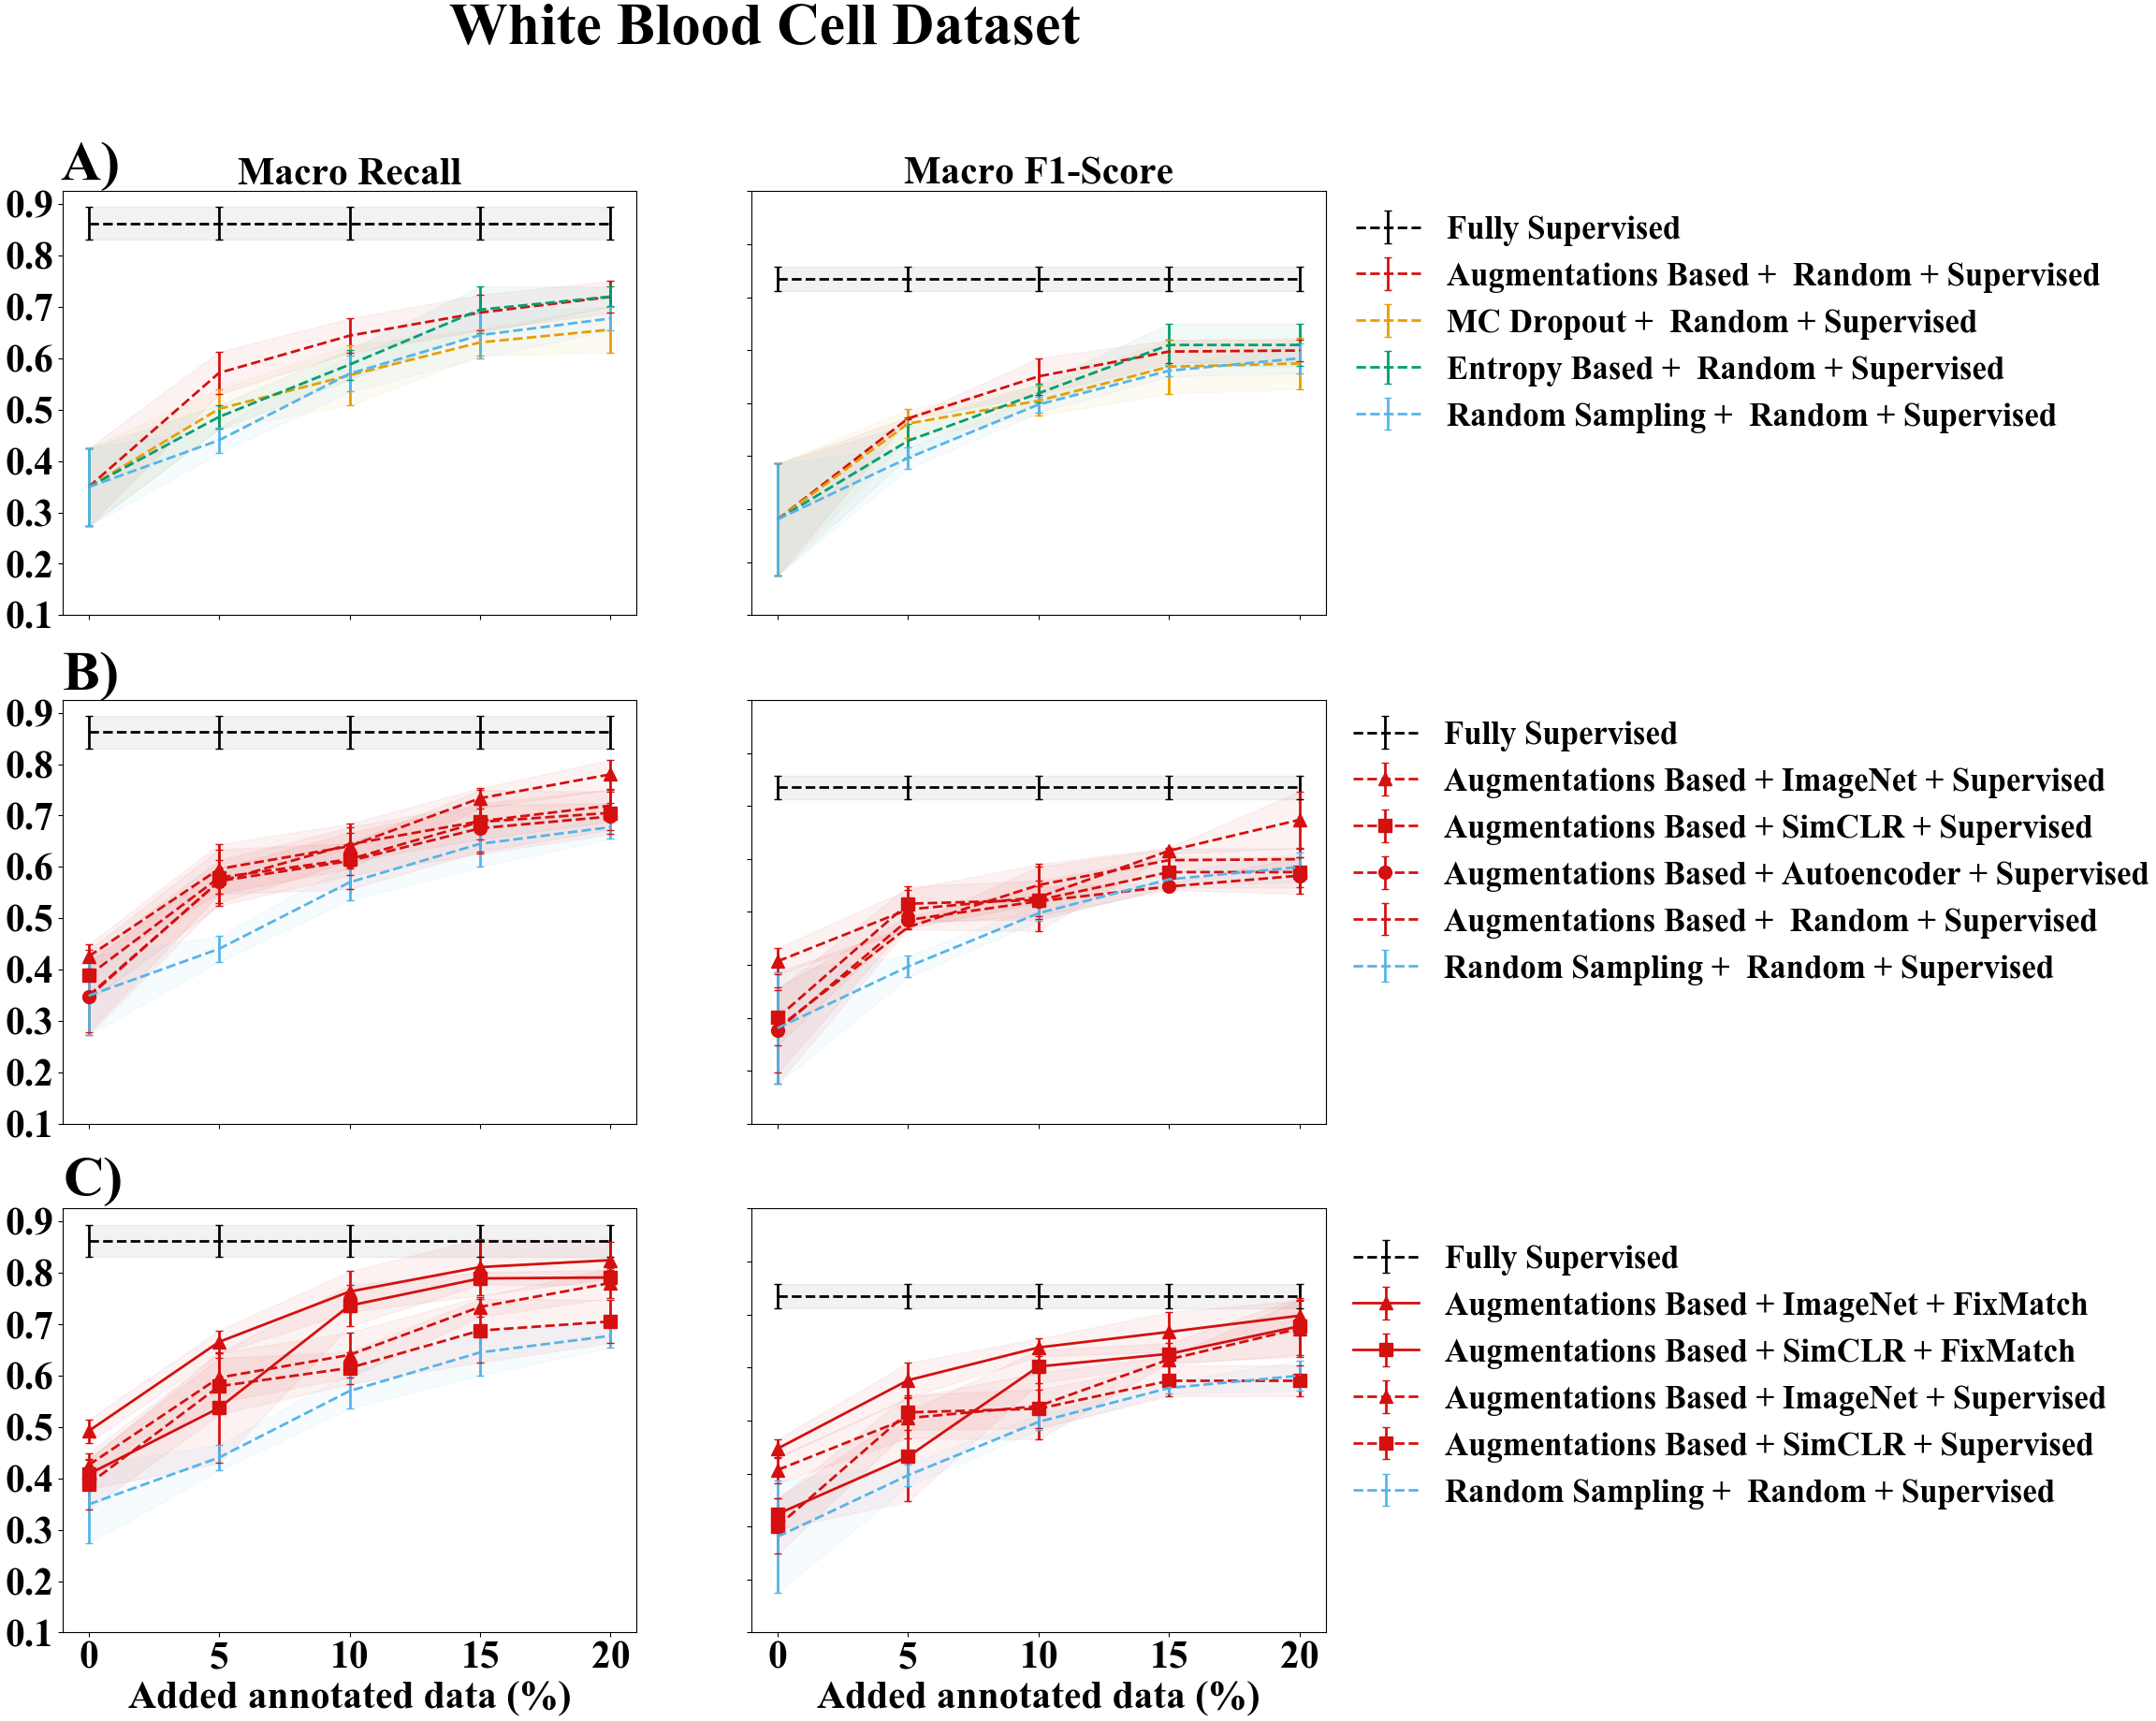
\includegraphics[width=\textwidth]{figures/fig_2_white_recall_f1.png}
\caption{On the white blood cell dataset, combining augmentation-based sampling, ImageNet pre-training and semi-supervised learning via FixMatch converges to the performance of fully-supervised learning. (A) Macro recall for 3 different active learning algorithms is computed, including augmentation-based sampling (dashed red line) entropy-based sampling (dashed green line), and MC-dropout (dashed yellow line) and a comparison is made to random sampling (dashed blue line). 1\% of the data is used as the initial labeled set. In each iteration, 5\% of data is added to the labeled set. Mean $\pm$ standard deviation of the macro recall is shown after 4-fold cross-validation. (B) Augmentation-based sampling (dashed red line, as in A) is chosen as the best active learning algorithm and a comparison is made using different pre-training methods including ImageNet weights (triangle), SimCLR (square), and autoencoder (circle) with random initialization (dashed blue line). (C) To study the effect of semi-supervised learning, the best performing experiments from B are repeated using FixMatch.}
\label{fig:fig_2_white_recall_f1}
\end{figure}

\begin{figure}[htbp]
\centering
\captionsetup{format=plain}
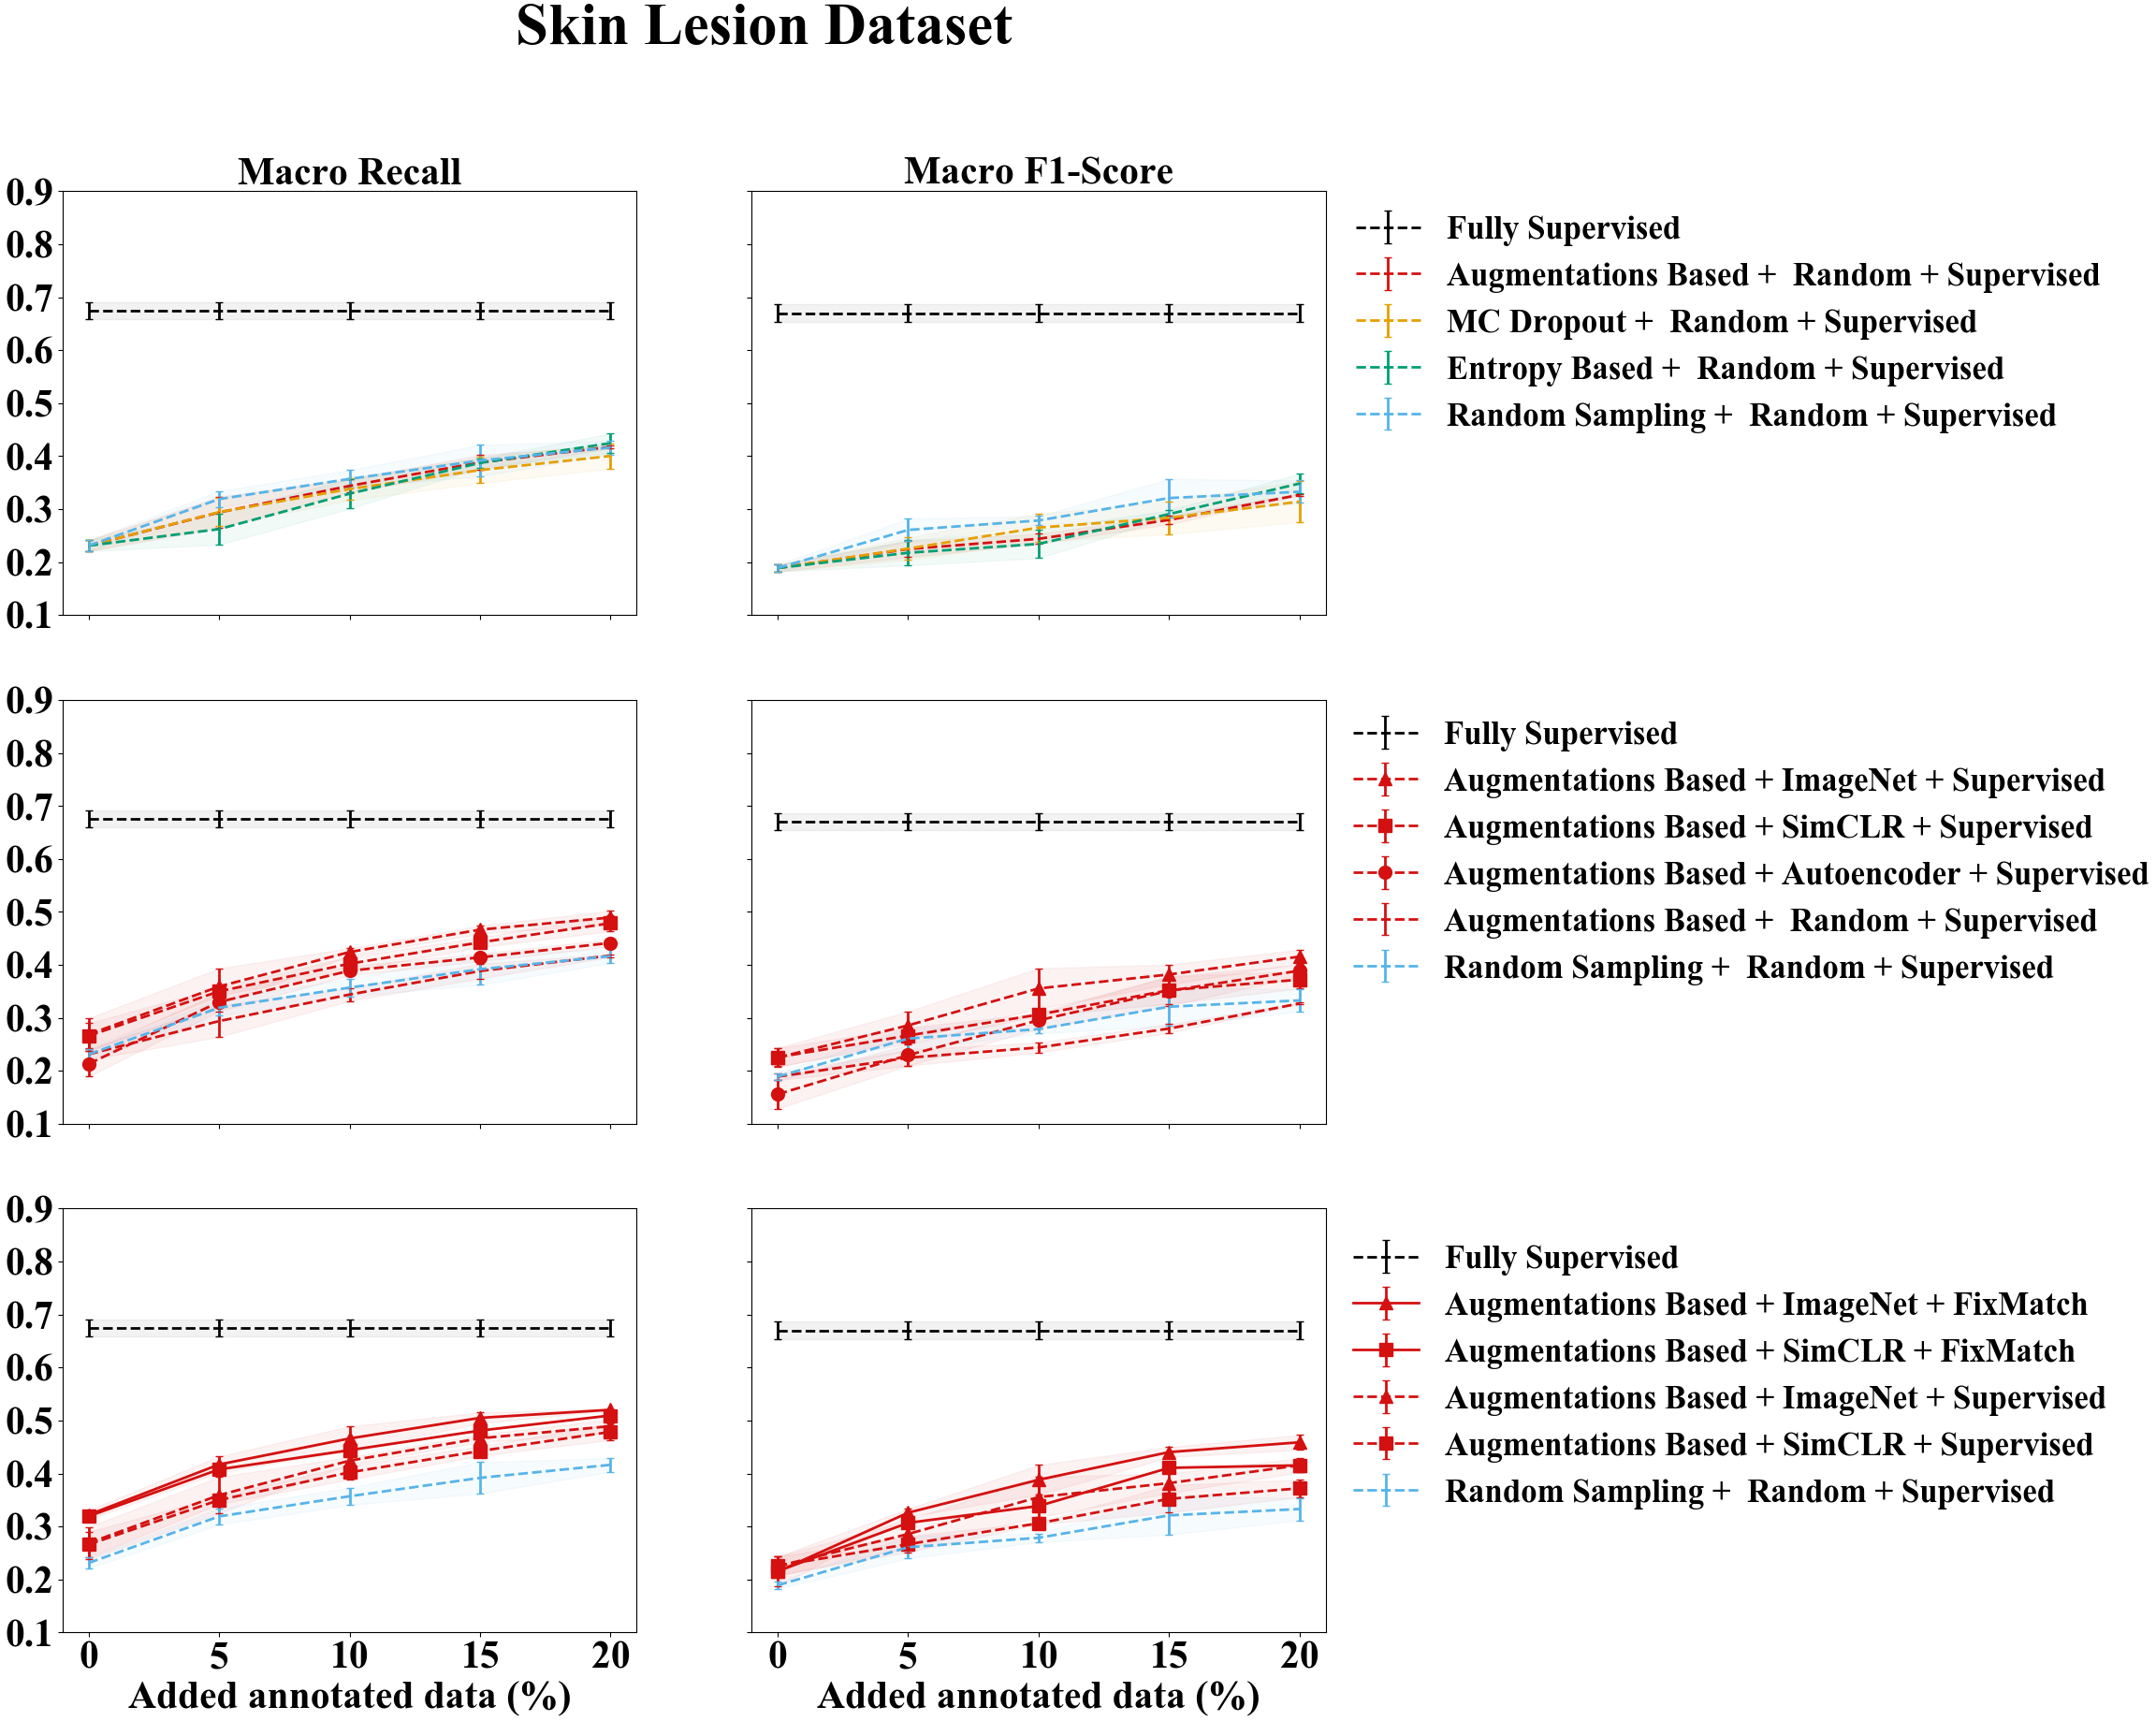
\includegraphics[width=\textwidth]{figures/fig_2_skin_recall_f1.png}
\caption{On the white blood cell dataset, combining augmentation-based sampling, ImageNet pre-training and semi-supervised learning via FixMatch converges to the performance of fully-supervised learning. (A) Macro recall for 3 different active learning algorithms is computed, including augmentation-based sampling (dashed red line) entropy-based sampling (dashed green line), and MC-dropout (dashed yellow line) and a comparison is made to random sampling (dashed blue line). 1\% of the data is used as the initial labeled set. In each iteration, 5\% of data is added to the labeled set. Mean $\pm$ standard deviation of the macro recall is shown after 4-fold cross-validation. (B) Augmentation-based sampling (dashed red line, as in A) is chosen as the best active learning algorithm and a comparison is made using different pre-training methods including ImageNet weights (triangle), SimCLR (square), and autoencoder (circle) with random initialization (dashed blue line). (C) To study the effect of semi-supervised learning, the best performing experiments from B are repeated using FixMatch.}
\label{fig:fig_2_skin_recall_f1}
\end{figure}

\begin{figure}[htbp]
\centering
\captionsetup{format=plain}
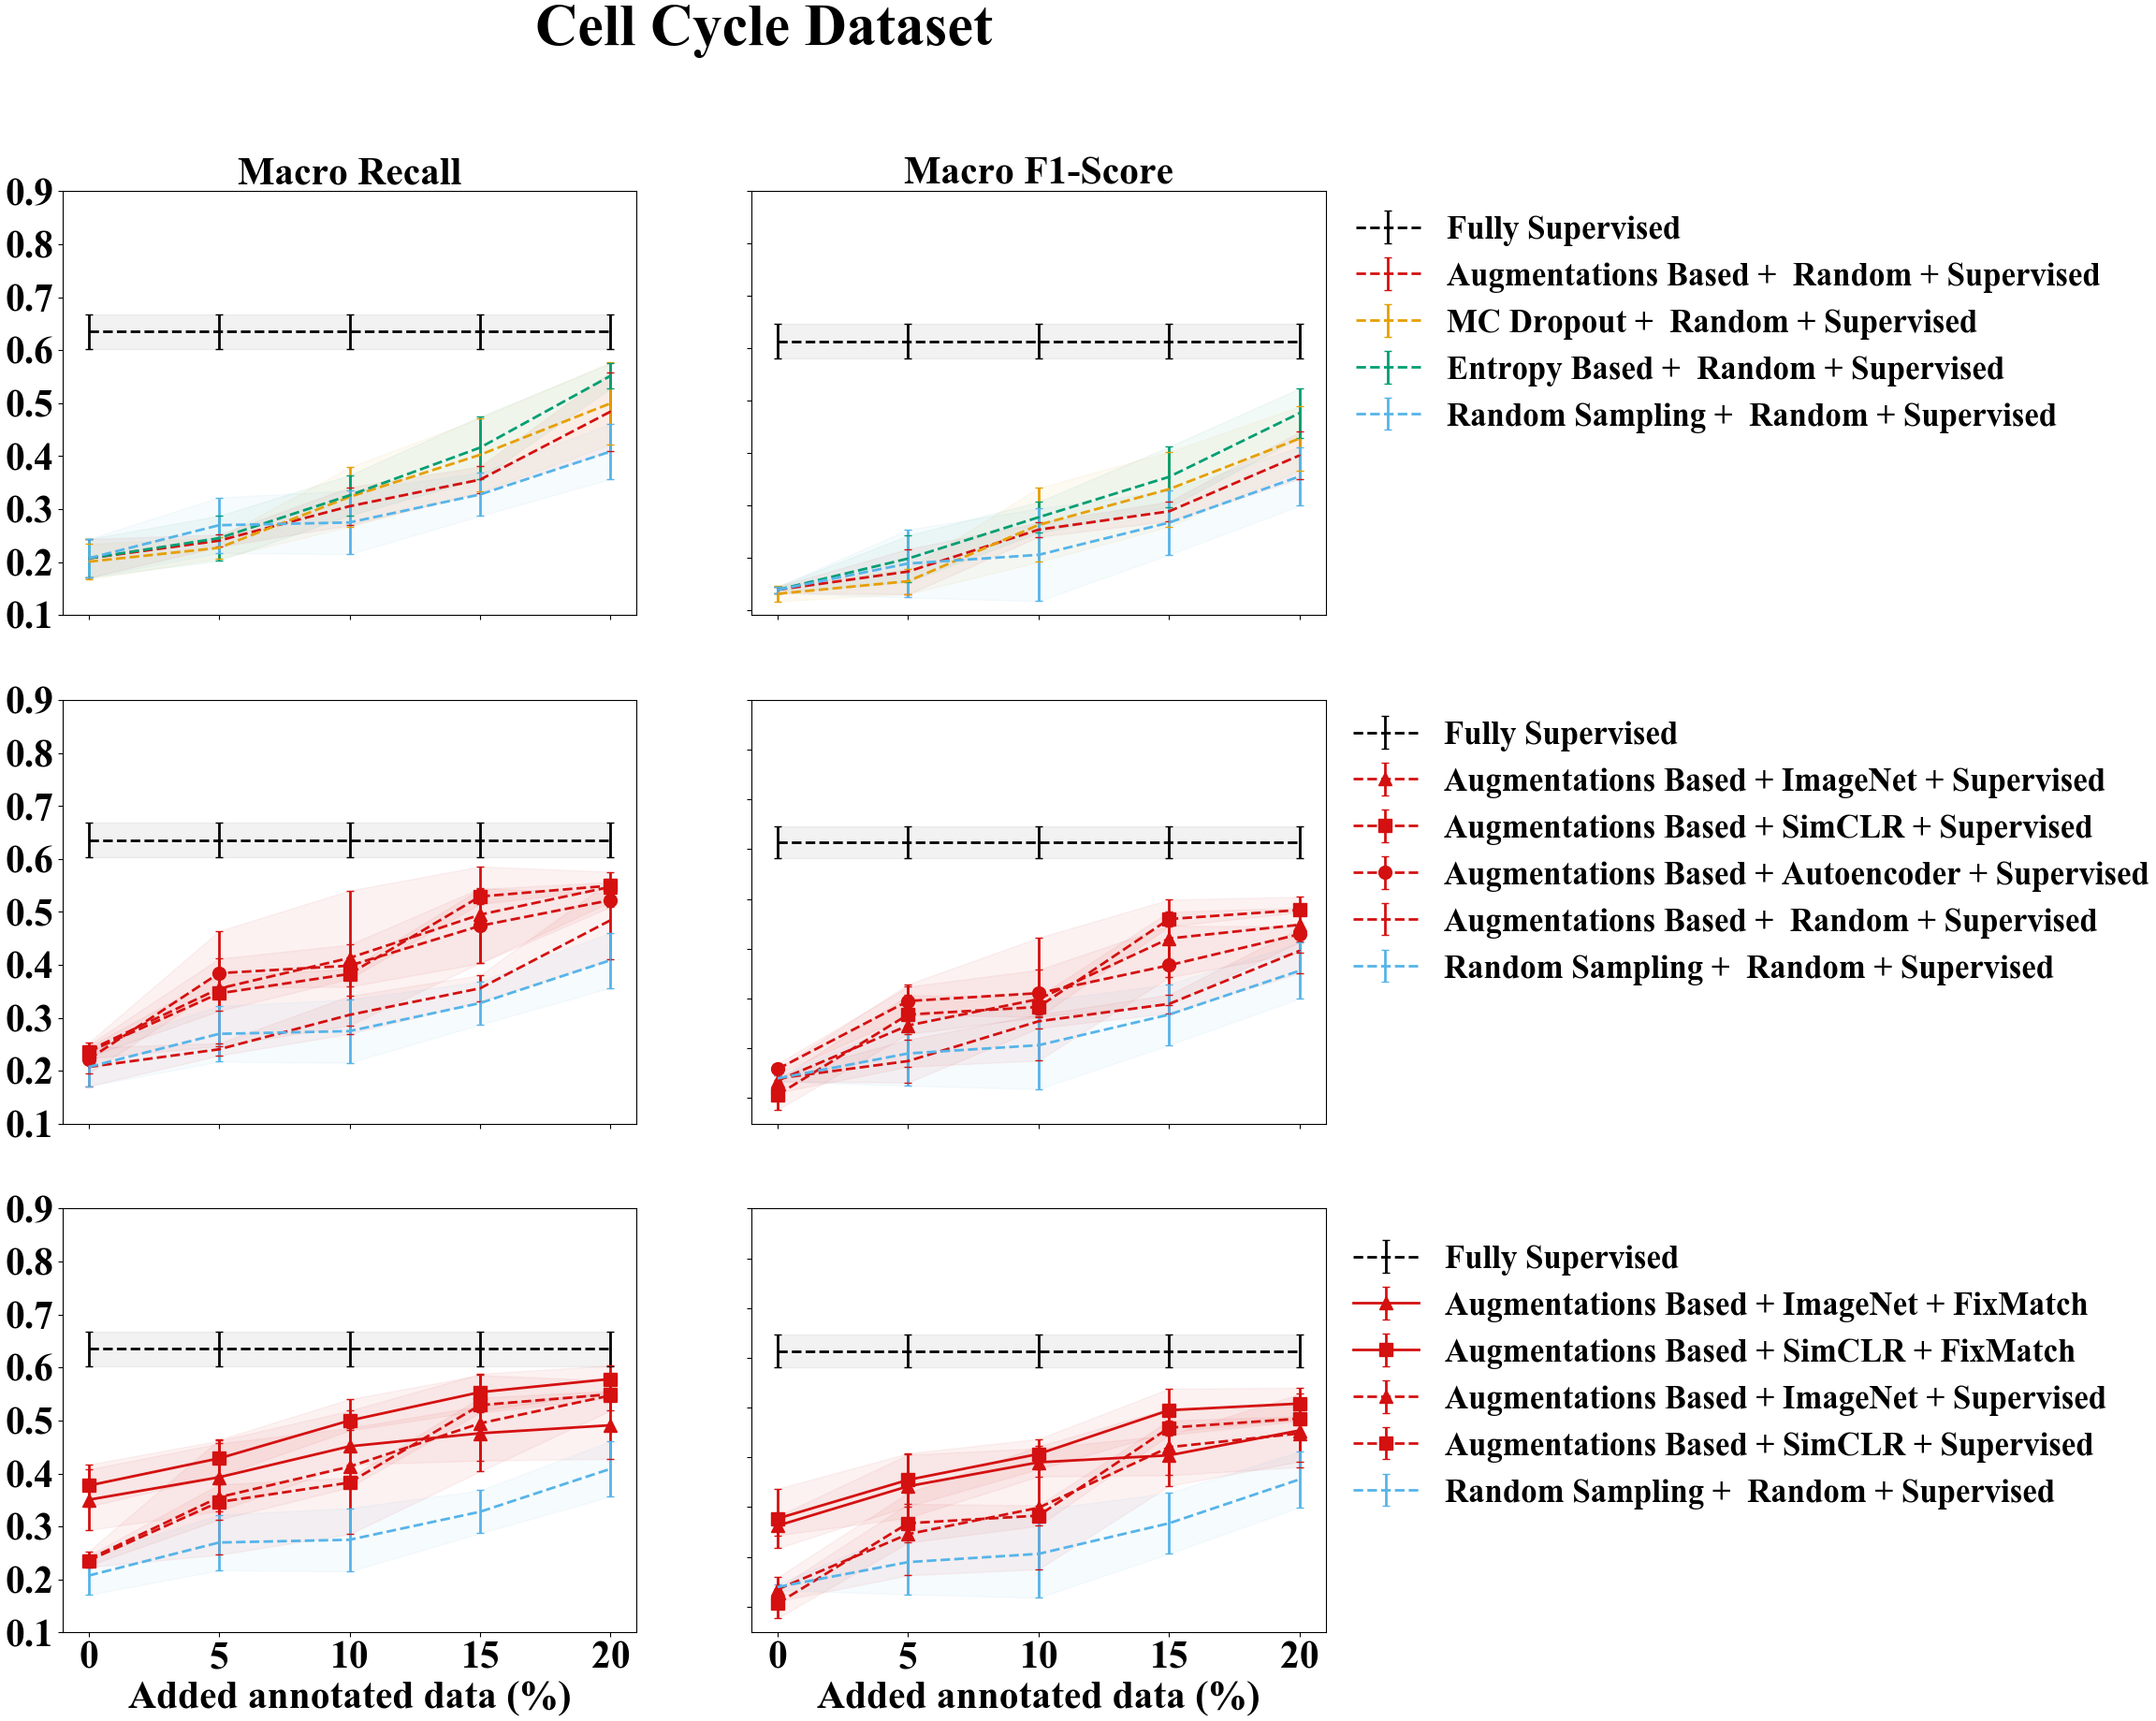
\includegraphics[width=\textwidth]{figures/fig_2_cycle_recall_f1.png}
\caption{On the white blood cell dataset, combining augmentation-based sampling, ImageNet pre-training and semi-supervised learning via FixMatch converges to the performance of fully-supervised learning. (A) Macro recall for 3 different active learning algorithms is computed, including augmentation-based sampling (dashed red line) entropy-based sampling (dashed green line), and MC-dropout (dashed yellow line) and a comparison is made to random sampling (dashed blue line). 1\% of the data is used as the initial labeled set. In each iteration, 5\% of data is added to the labeled set. Mean $\pm$ standard deviation of the macro recall is shown after 4-fold cross-validation. (B) Augmentation-based sampling (dashed red line, as in A) is chosen as the best active learning algorithm and a comparison is made using different pre-training methods including ImageNet weights (triangle), SimCLR (square), and autoencoder (circle) with random initialization (dashed blue line). (C) To study the effect of semi-supervised learning, the best performing experiments from B are repeated using FixMatch.}
\label{fig:fig_2_cycle_recall_f1}
\end{figure}

\begin{figure}[htbp]
\centering
\captionsetup{format=plain}
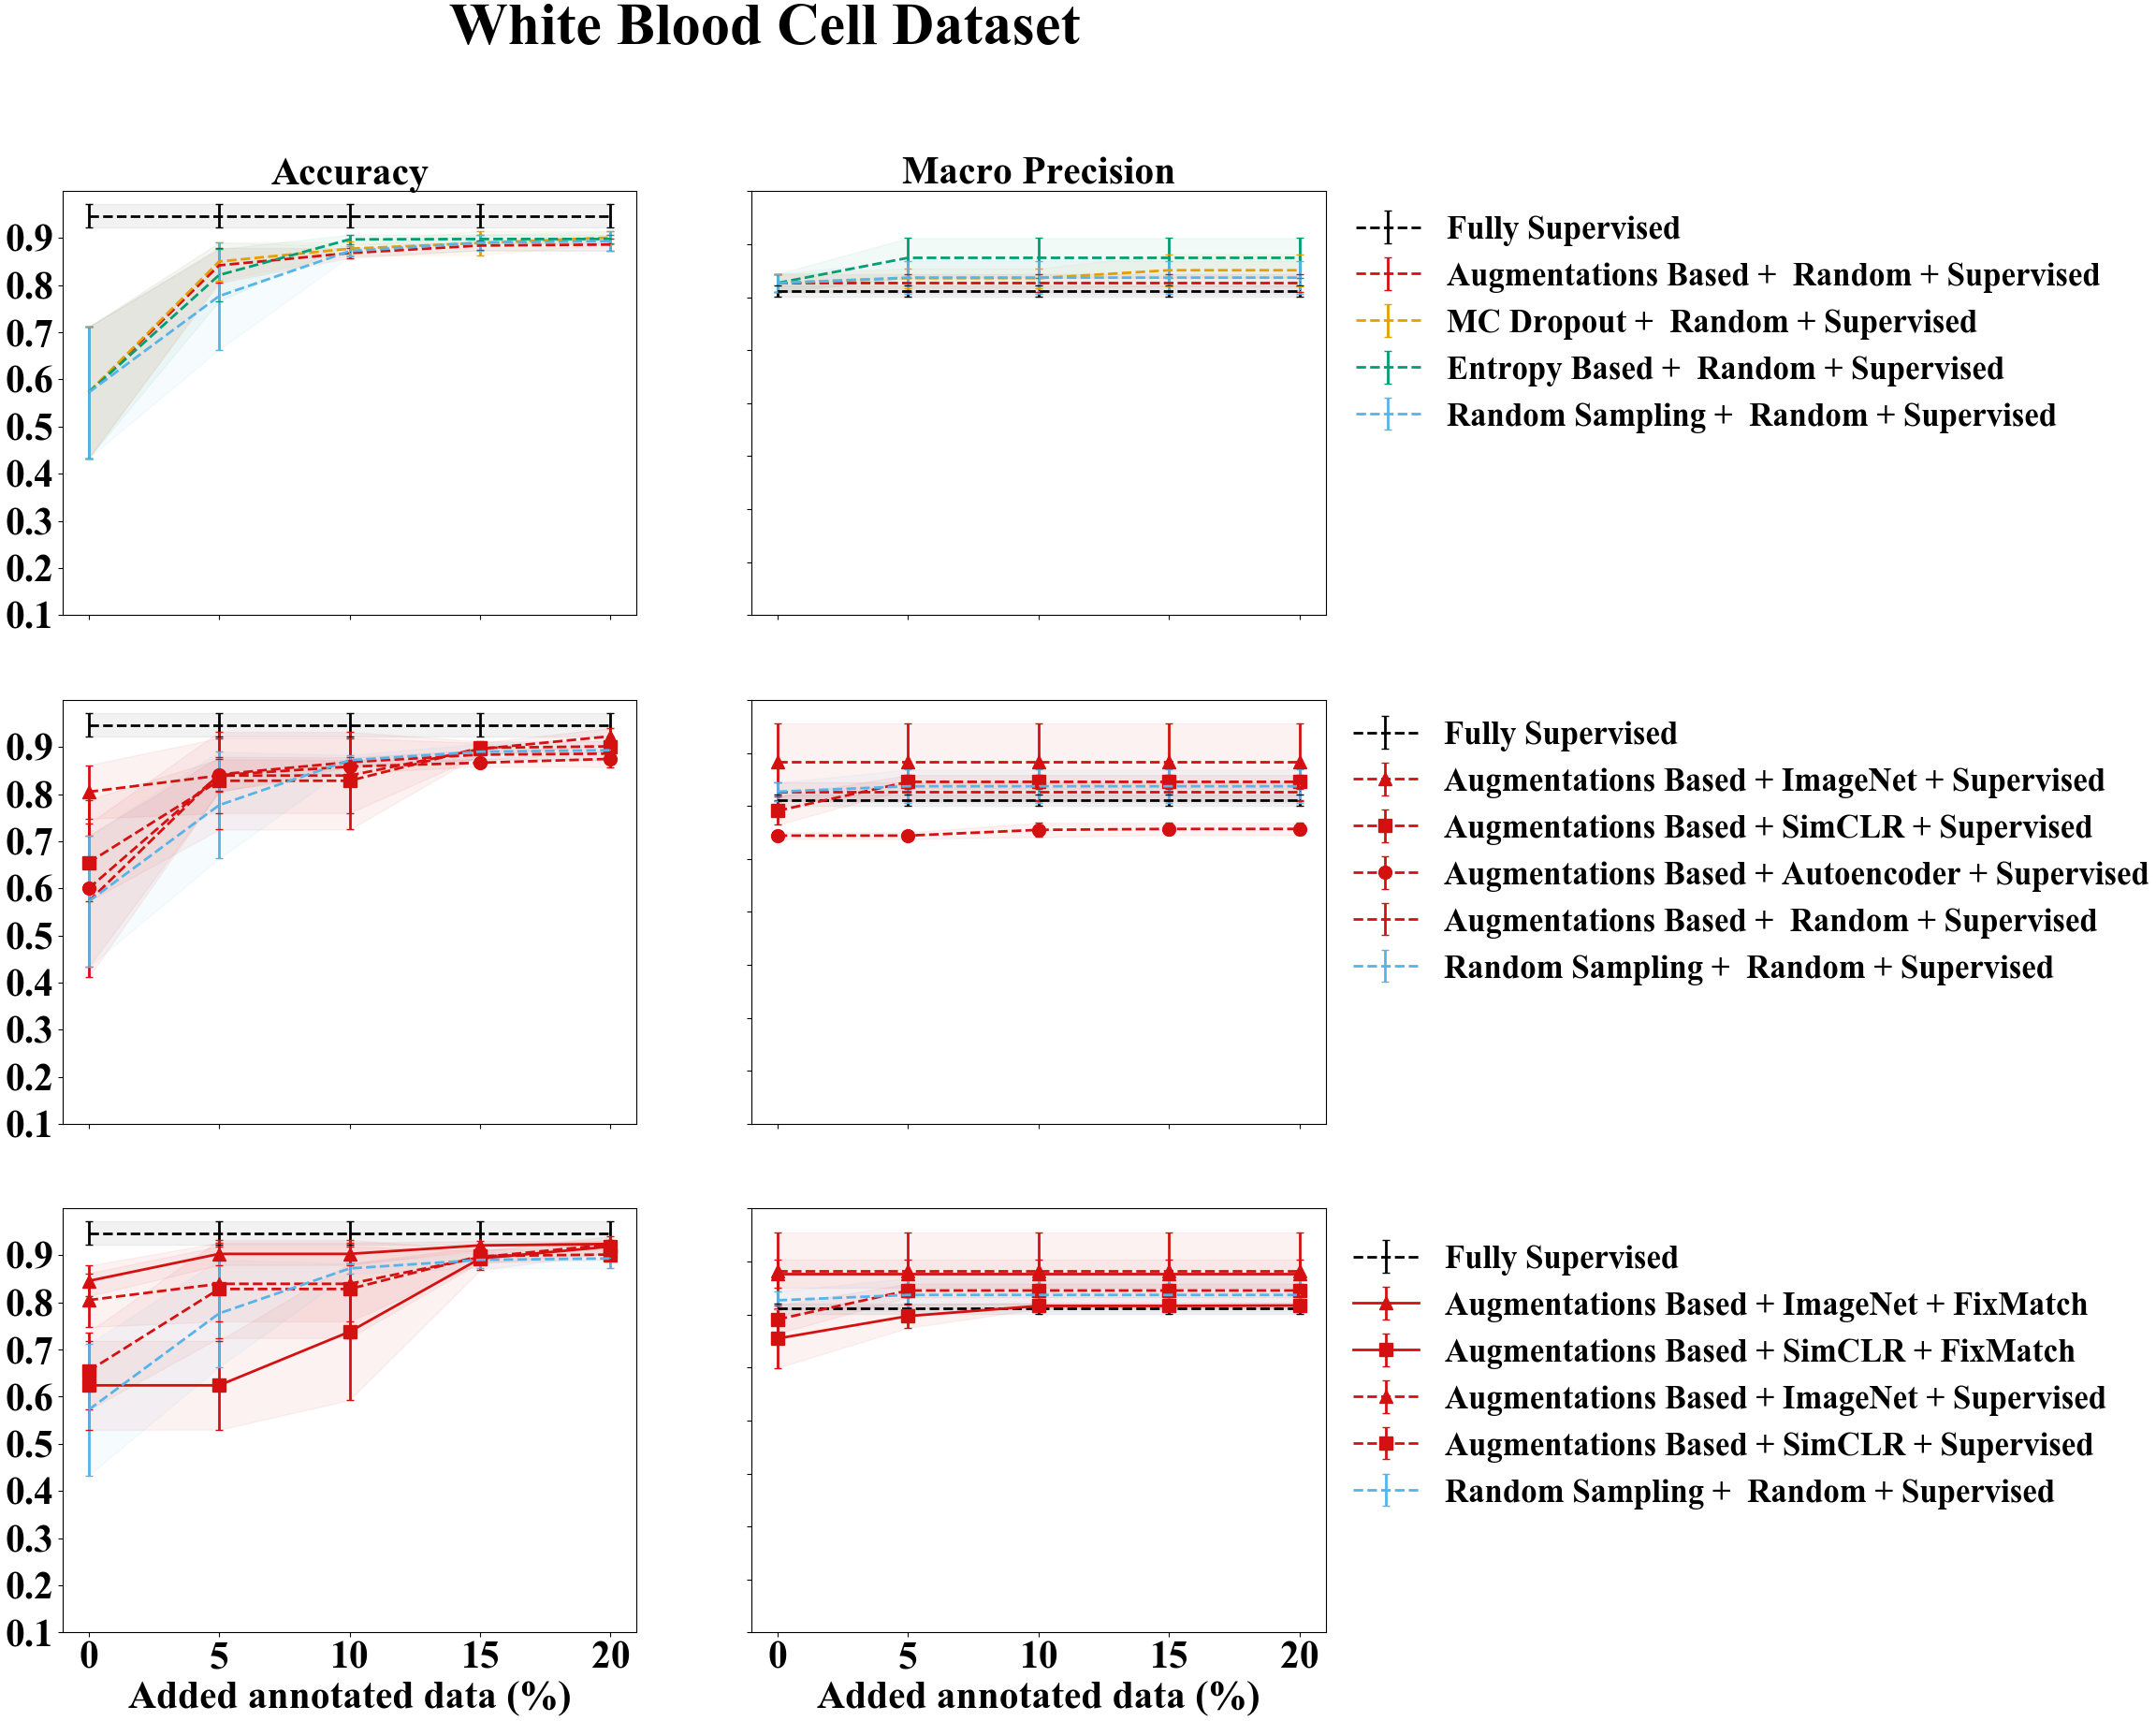
\includegraphics[width=\textwidth]{figures/fig_2_white_acc_precision.png}
\caption{On the white blood cell dataset, combining augmentation-based sampling, ImageNet pre-training and semi-supervised learning via FixMatch converges to the performance of fully-supervised learning. (A) Macro recall for 3 different active learning algorithms is computed, including augmentation-based sampling (dashed red line) entropy-based sampling (dashed green line), and MC-dropout (dashed yellow line) and a comparison is made to random sampling (dashed blue line). 1\% of the data is used as the initial labeled set. In each iteration, 5\% of data is added to the labeled set. Mean $\pm$ standard deviation of the macro recall is shown after 4-fold cross-validation. (B) Augmentation-based sampling (dashed red line, as in A) is chosen as the best active learning algorithm and a comparison is made using different pre-training methods including ImageNet weights (triangle), SimCLR (square), and autoencoder (circle) with random initialization (dashed blue line). (C) To study the effect of semi-supervised learning, the best performing experiments from B are repeated using FixMatch.}
\label{fig:fig_2_white_acc_precision}
\end{figure}

\begin{figure}[htbp]
\centering
\captionsetup{format=plain}
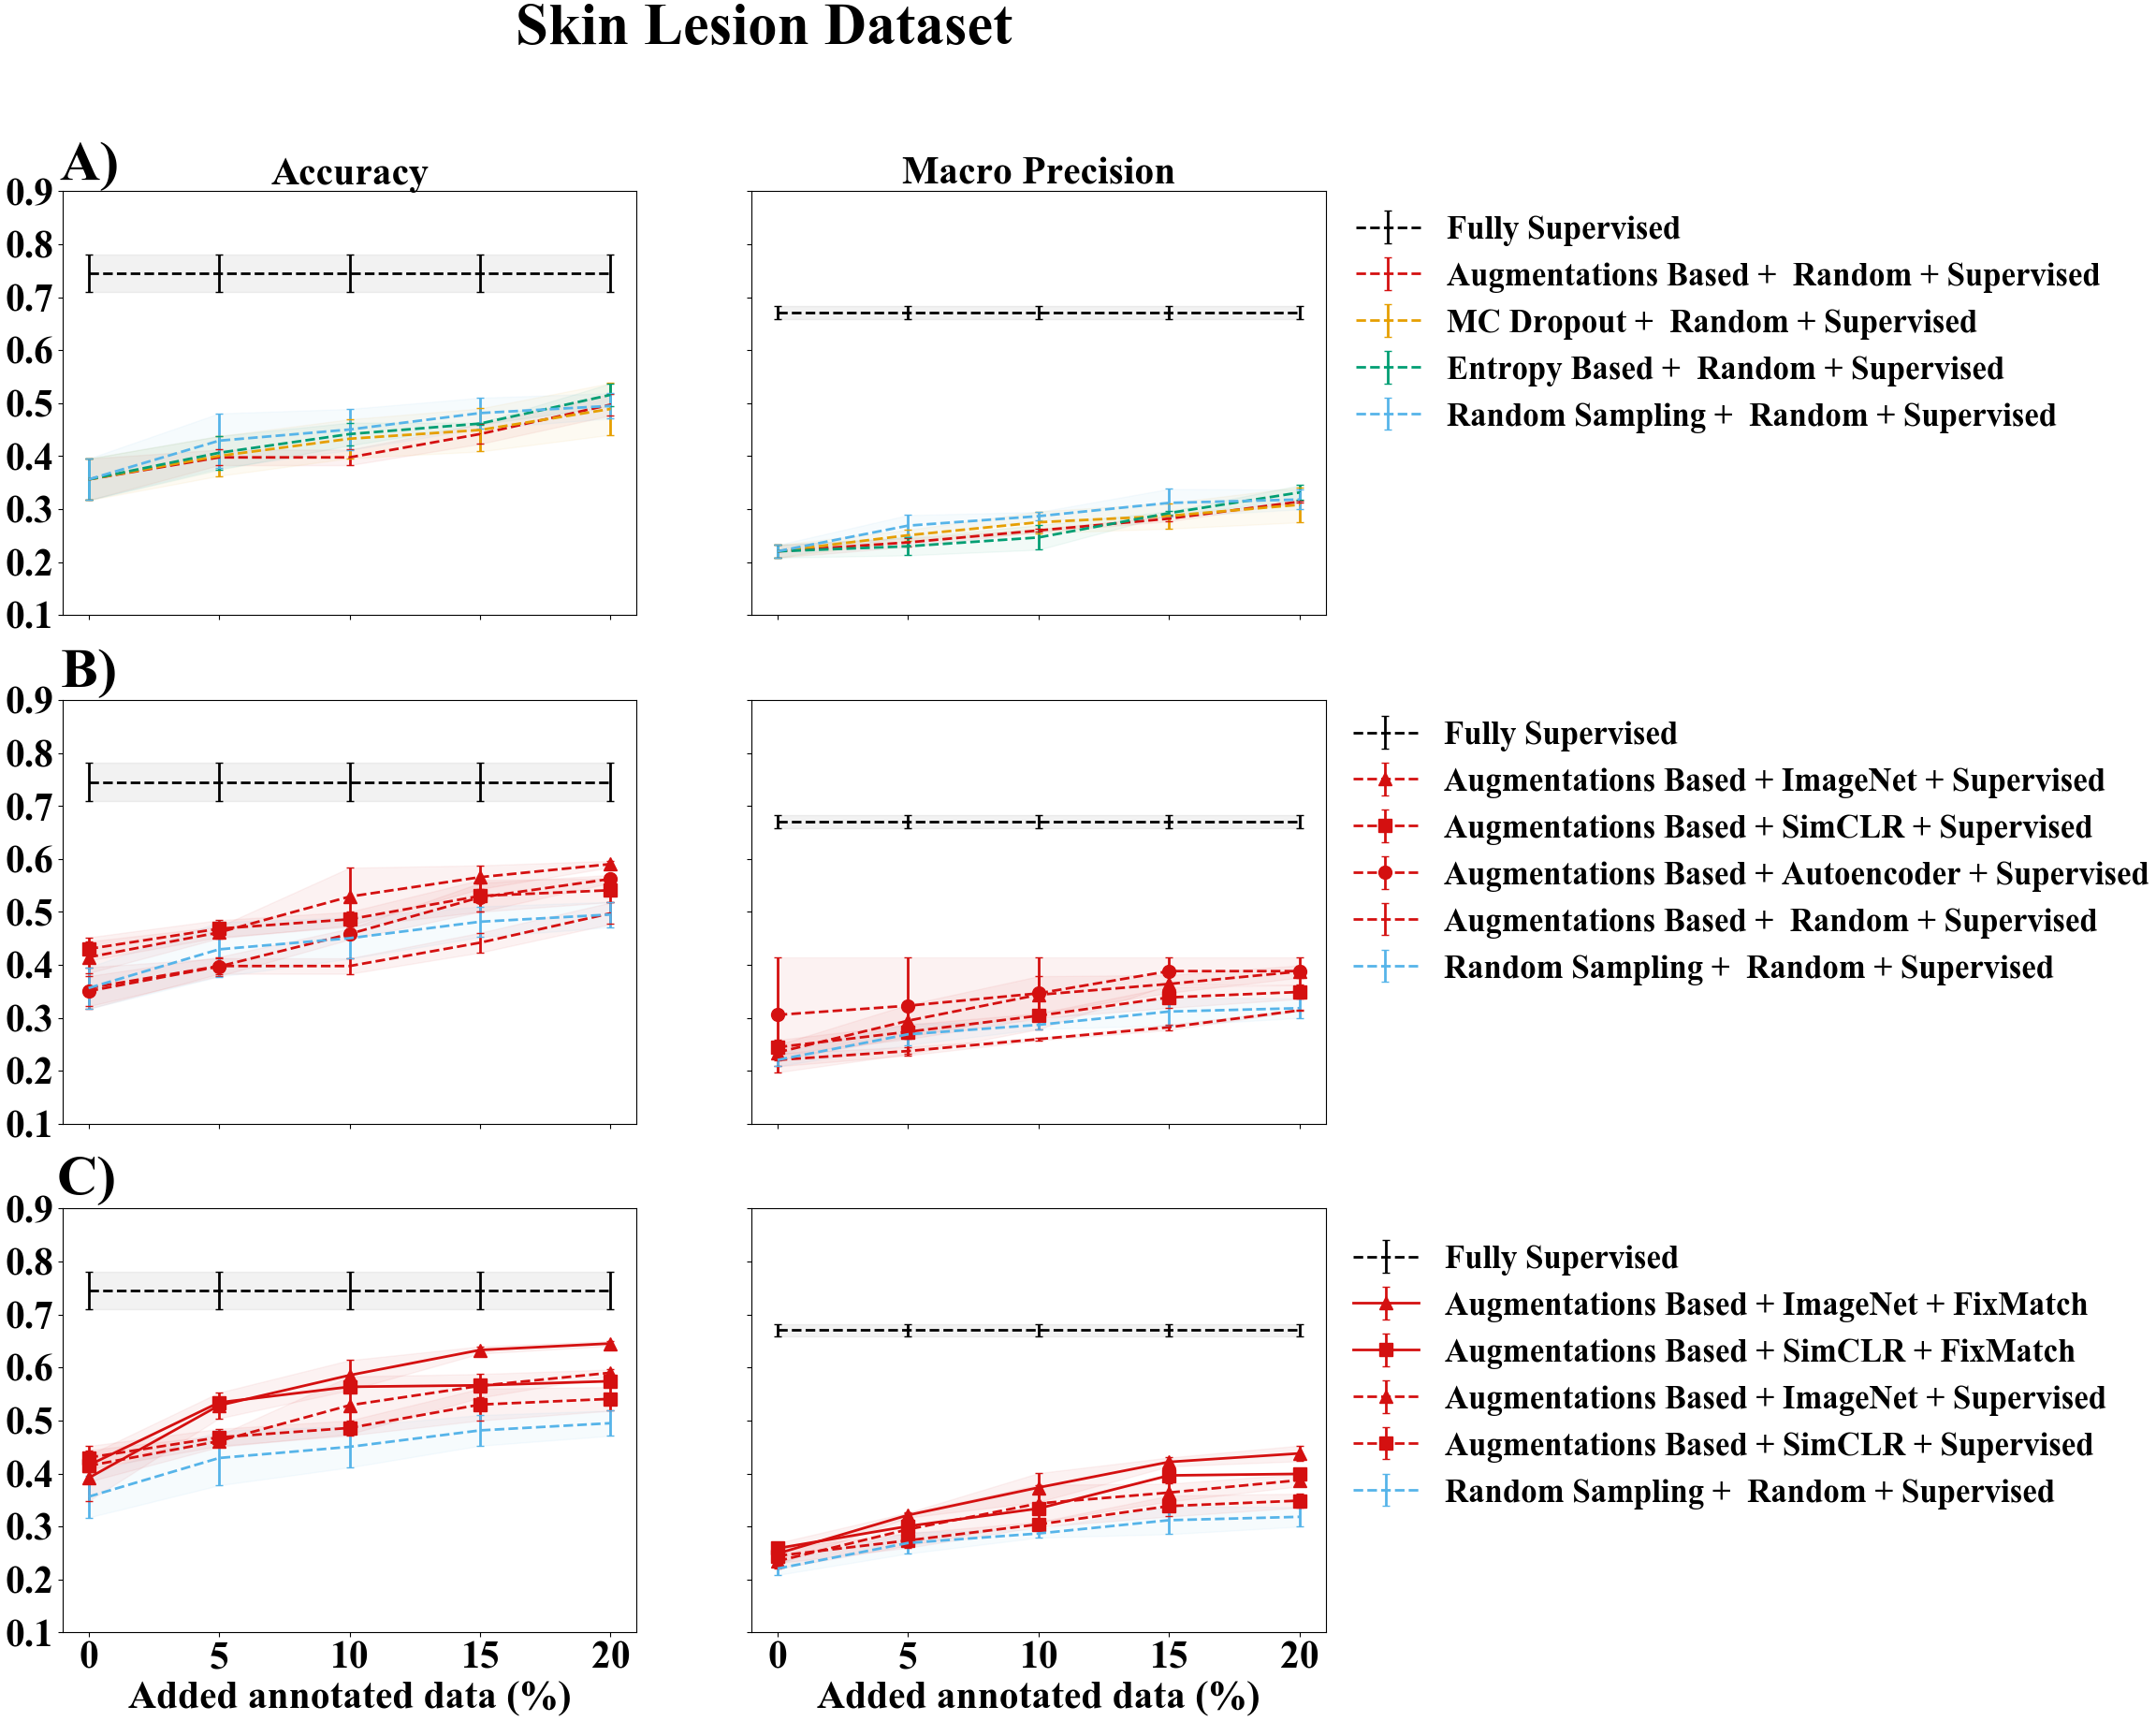
\includegraphics[width=\textwidth]{figures/fig_2_skin_acc_precision.png}
\caption{On the white blood cell dataset, combining augmentation-based sampling, ImageNet pre-training and semi-supervised learning via FixMatch converges to the performance of fully-supervised learning. (A) Macro recall for 3 different active learning algorithms is computed, including augmentation-based sampling (dashed red line) entropy-based sampling (dashed green line), and MC-dropout (dashed yellow line) and a comparison is made to random sampling (dashed blue line). 1\% of the data is used as the initial labeled set. In each iteration, 5\% of data is added to the labeled set. Mean $\pm$ standard deviation of the macro recall is shown after 4-fold cross-validation. (B) Augmentation-based sampling (dashed red line, as in A) is chosen as the best active learning algorithm and a comparison is made using different pre-training methods including ImageNet weights (triangle), SimCLR (square), and autoencoder (circle) with random initialization (dashed blue line). (C) To study the effect of semi-supervised learning, the best performing experiments from B are repeated using FixMatch.}
\label{fig:fig_2_skin_acc_precision}
\end{figure}

\begin{figure}[htbp]
\centering
\captionsetup{format=plain}
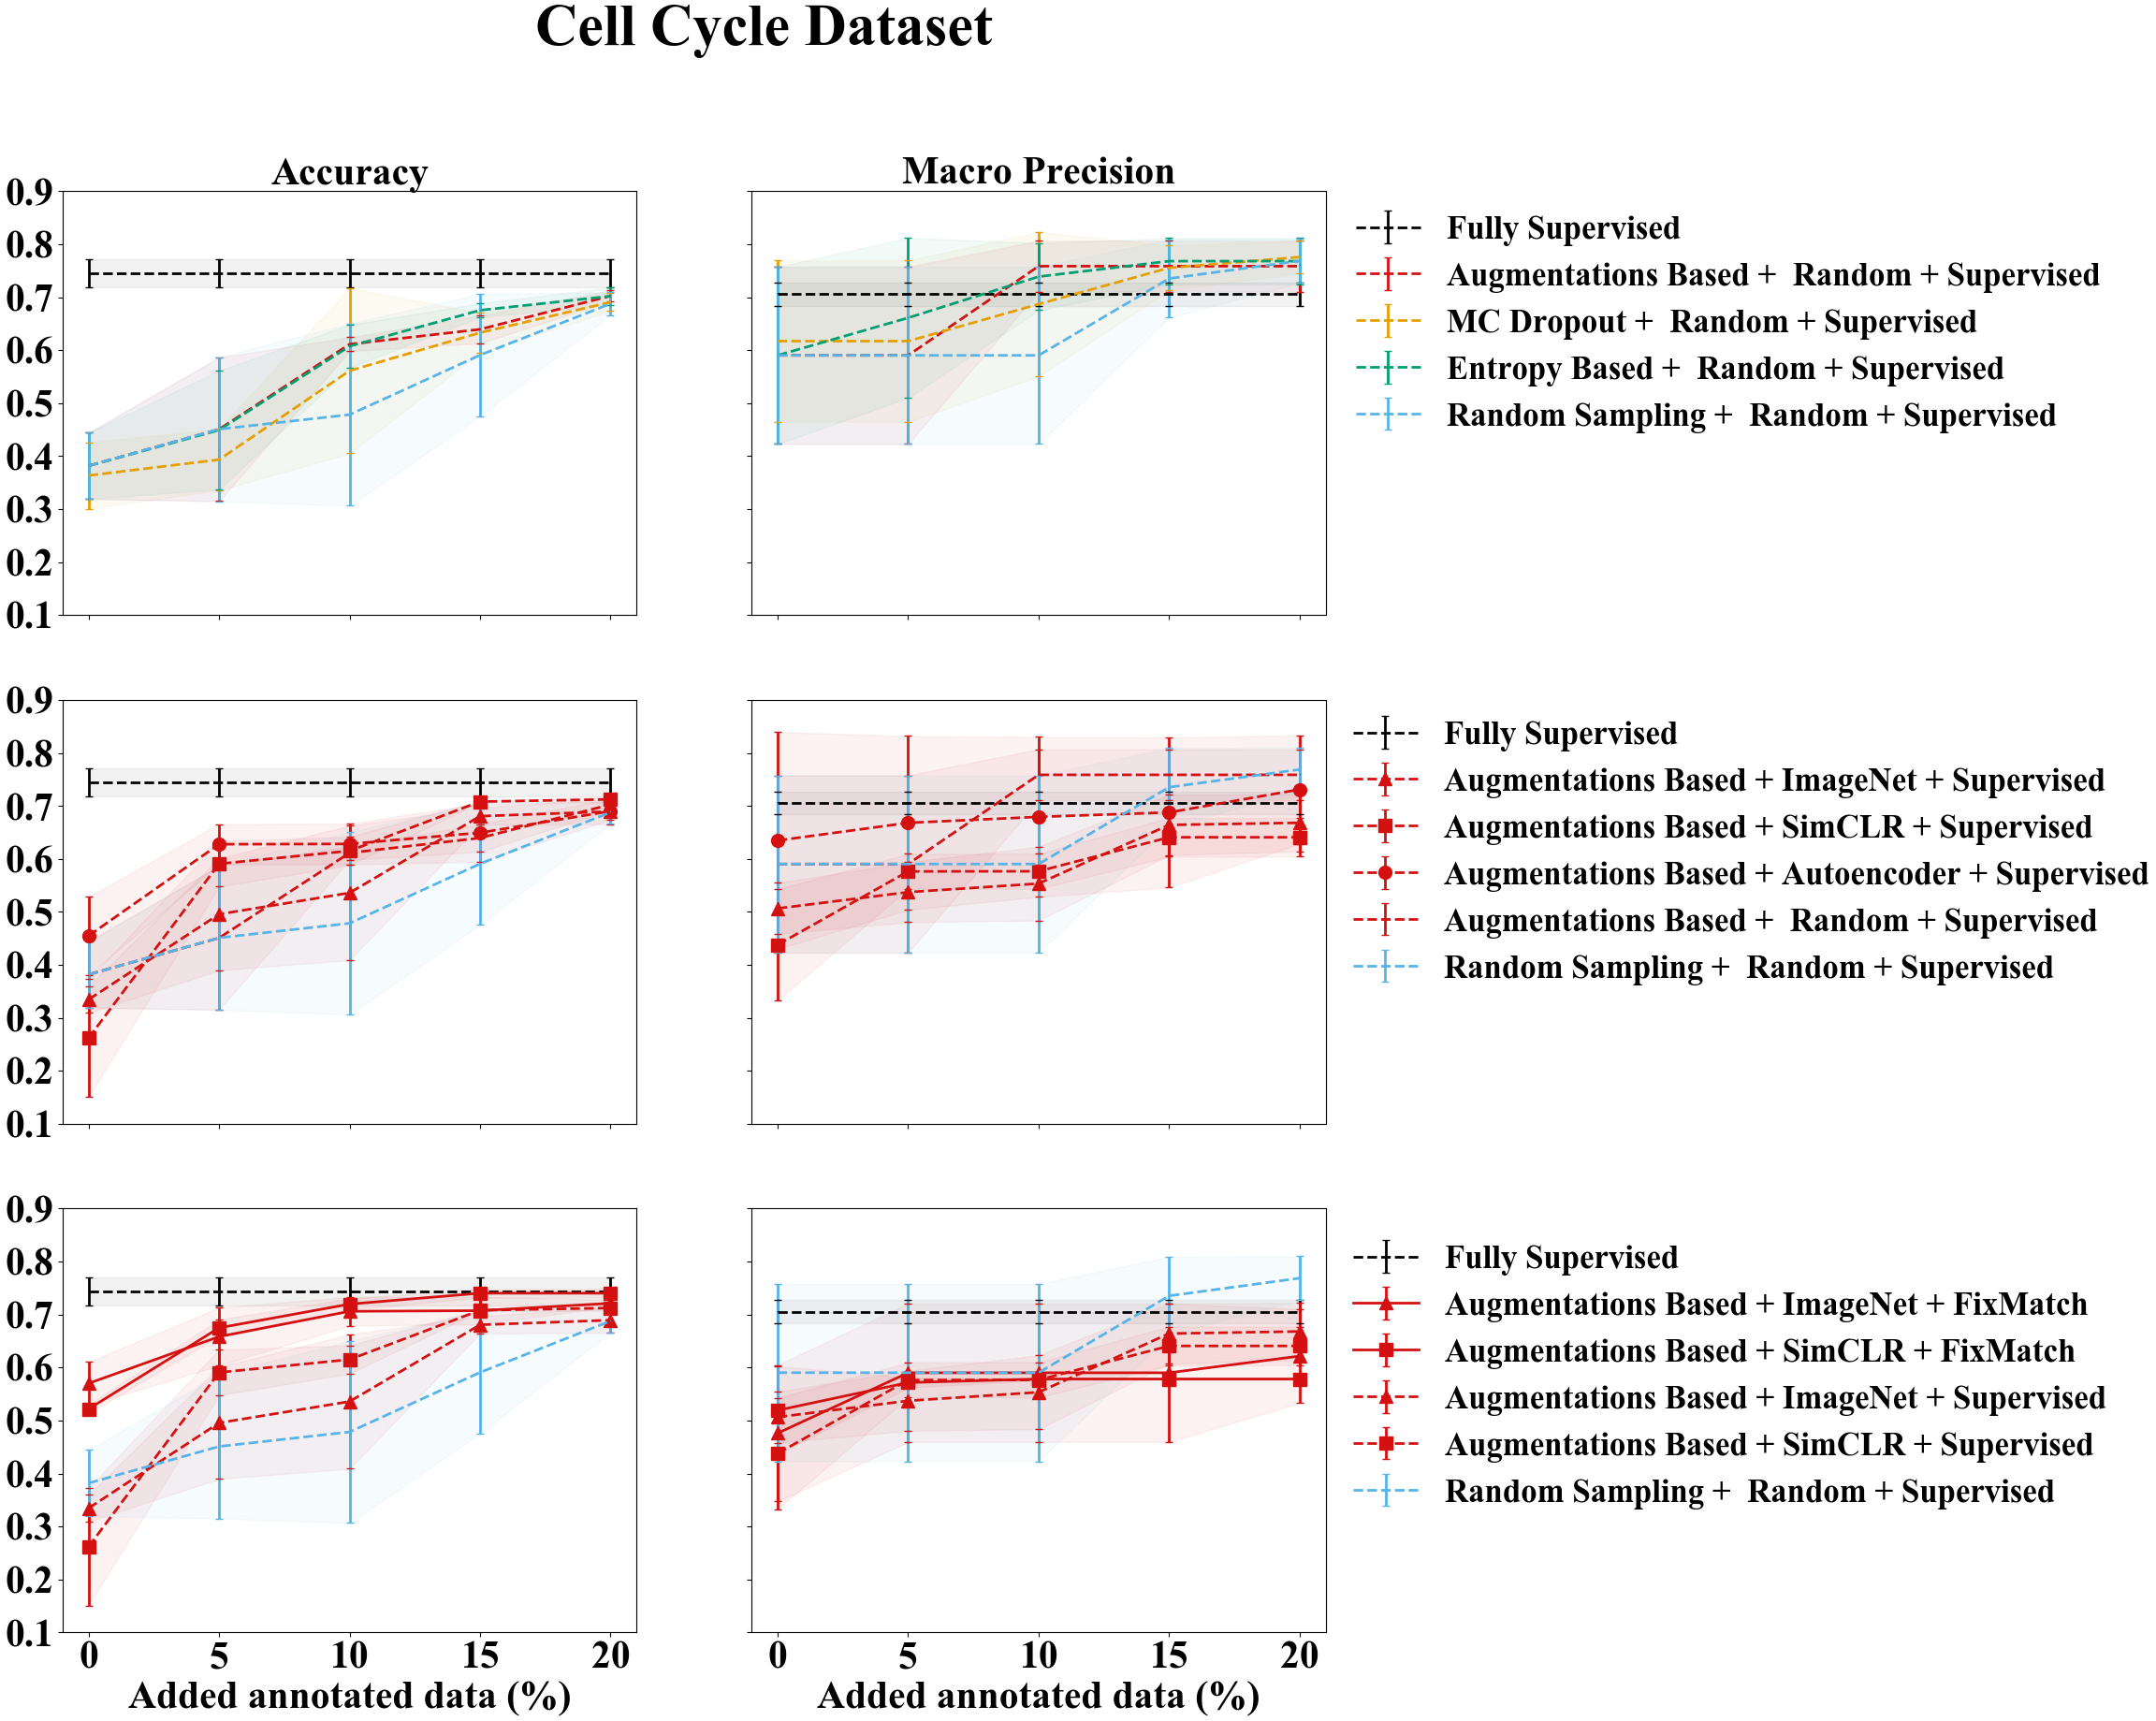
\includegraphics[width=\textwidth]{figures/fig_2_cycle_acc_precision.png}
\caption{On the white blood cell dataset, combining augmentation-based sampling, ImageNet pre-training and semi-supervised learning via FixMatch converges to the performance of fully-supervised learning. (A) Macro recall for 3 different active learning algorithms is computed, including augmentation-based sampling (dashed red line) entropy-based sampling (dashed green line), and MC-dropout (dashed yellow line) and a comparison is made to random sampling (dashed blue line). 1\% of the data is used as the initial labeled set. In each iteration, 5\% of data is added to the labeled set. Mean $\pm$ standard deviation of the macro recall is shown after 4-fold cross-validation. (B) Augmentation-based sampling (dashed red line, as in A) is chosen as the best active learning algorithm and a comparison is made using different pre-training methods including ImageNet weights (triangle), SimCLR (square), and autoencoder (circle) with random initialization (dashed blue line). (C) To study the effect of semi-supervised learning, the best performing experiments from B are repeated using FixMatch.}
\label{fig:fig_2_cycle_acc_precision}
\end{figure}

\section{Comparison of active learning algorithms on white blood cell data}
First, the performance of different annotation-efficient approaches is compared on the white blood cell dataset (Figure \ref{fig:fig_2_white_recall_f1}). Random Initialization is used for model weights initialization and the model is trained under the supervised learning paradigm i.e. using labeled data only. The augmentation-based sampling achieves better performance compared to all other active learning algorithms (see Figure \ref{fig:results_3}) in almost all active learning iterations (see Figure \ref{fig:fig_2_white_recall_f1}). At the last active learning iteration, after 20\% of data has already been added to the labeled set $\mathcal{L}$ as annotated images, the augmentation-based sampling has a macro recall of 0.72$\pm$0.03, entropy-based sampling a macro recall of 0.72$\pm$0.02, MC-dropout a recall of 0.66$\pm$0.04 and random sampling a recall of 0.68$\pm$0.02.

\section{Pre-training on white blood cell images further improves performance}
Augmentation-based sampling is the best performing active learning algorithm. The performance obtained through augmentation sampling is further improved by adding pre-training (Figure \ref{fig:fig_2_white_recall_f1}). Using augmentation-based sampling as the active learning algorithm, the experiment is repeated with three pre-training methods: using pre-trained ImageNet weights, using Autoencoder and using SimCLR (see chapter \ref{chapter:methods} and Table \ref{table:experimental_grid}). It is found that using pre-trained ImageNet  weights and SimCLR for pre-training results in a boost in performance in the first two active learning iterations with a increase of 12\% of macro recall. However, as more annotated data is added, the random initialization catches up with SimCLR and autoencoder pre-training but ImageNet pre-training still performs better than random initialization even after the addition of 20\% of the data. After the last active learning iteration, the  augmentation-based sampling with ImageNet weights reaches a macro recall of 0.78$\pm$0.03, random initialization reaches a macro recall of 0.72$\pm$0.03 and initialization with SimCLR pre-training reaches a recall of 0.71$\pm$0.04.

\section{Semi-supervised learning further improves recall for white blood cells data}
As augmentation-based sampling performed better than other active learning algorithms, it is chosen for further investigation to find out the performance improvement gained by using semi-supervised learning training strategy (Figure \ref{fig:fig_2_white_recall_f1}). The pre-training methods of using pre-trained ImageNet weights and SimCLR are used, as both of the methods performed well during the previous experiments (Figure \ref{fig:fig_2_white_recall_f1}B). For semi-supervised learning, FixMatch is used (Figure \ref{fig:fig_2_white_recall_f1}C). After adding semi-supervised learning with augmentations, a macro recall improvement of at least 6\% is observed for all iterations. This combination performs better than supervised training in each iteration and achieves a macro recall of 0.82$\pm$0.04 at the last iteration, when 20\% of annotated data has been added to the labeled set $\mathcal{L}$. FixMatch also improves augmentation-based sampling with SimCLR pre-training, reaching 0.79$\pm$0.01 macro recall. It is to be noted that when using augmentation-based active learning algorithm with ImageNet pre-training and semi-supervised learning, the macro recall is only 4\% less than using fully-supervised learning on 100\% of the data.

\section{Grid-search identifies the best performing combinations for three biomedical datasets}
To investigation if the proposed combination of augmentation-based sampling, ImageNet pre-training and semi-supervised learning performs better than other combinations in table \ref{table:experimental_grid} for biomedical datasets which involve images containing different textures, colors and structures. The proposed combination is tested on three different biomedical datasets (Figure \ref{fig:datasets_composition}). For this purpose an extensive grid search is carried out which specifically involves, 3x4x4x2x4x5 = 1920 independent runs (3 datasets, 3 active learning algorithms plus random sampling, 3 pre-training methods plus random initialization, 2 training strategies, 4-fold cross-validation and 1 initial step plus 4 active learning iterations). The criteria for measuring the performance of different combinations is the macro recall value at the last iteration when 20\% of data has been added as annotated data.

It is found that the proposed combinations of augmentation-based sampling with ImageNet or SimCLR pre-training and FixMatch consistently outperform the rest (for comparing all the combinations, please refer to the appendix).
In case of white blood cell dataset, at the first step with 1\% of labeled data a 6\% improvement in macro recall at least is observed using FixMatch with ImageNet initialization over conventional training method with only labeled data (Figure \ref{fig:all_recall_f1}A). This improvement in performance is stable, resulting in at least 4\% increase in macro recall compared to the best result obtained through supervised learning training strategy. The same trend is observed in case of the skin lesion dataset (Figure \ref{fig:all_recall_f1}B). During the first iteration, an improvement of at least 5\% is observed compared to other supervised learning conventional methods. Although the conventional supervised learning methods approach the performance of proposed combinations as more data is added, there is still a performance gap at all iterations. Lastly, for the cell cycle dataset (Figure \ref{fig:all_recall_f1}C), the combination of SimCLR with augmentation-based sampling provides a boost of at least 16\% in the macro recall in the start over other conventional methods. The performance boost gets less as more data is added but till the last iteration when 20\% of data has been added as annotated data, the performance improvement is still at least 3\% of macro recall. 
It is to be noted that, at the last iteration, for white blood cell dataset and the cell cycle dataset, the performance of the propose combinations approach the performance of fully-supervised learning on the whole dataset. However, in case of skin lesion dataset, more labeled data has to be added to approach the performance of fully supervised learning. 

\begin{figure}[htbp]
\centering
\captionsetup{format=plain}
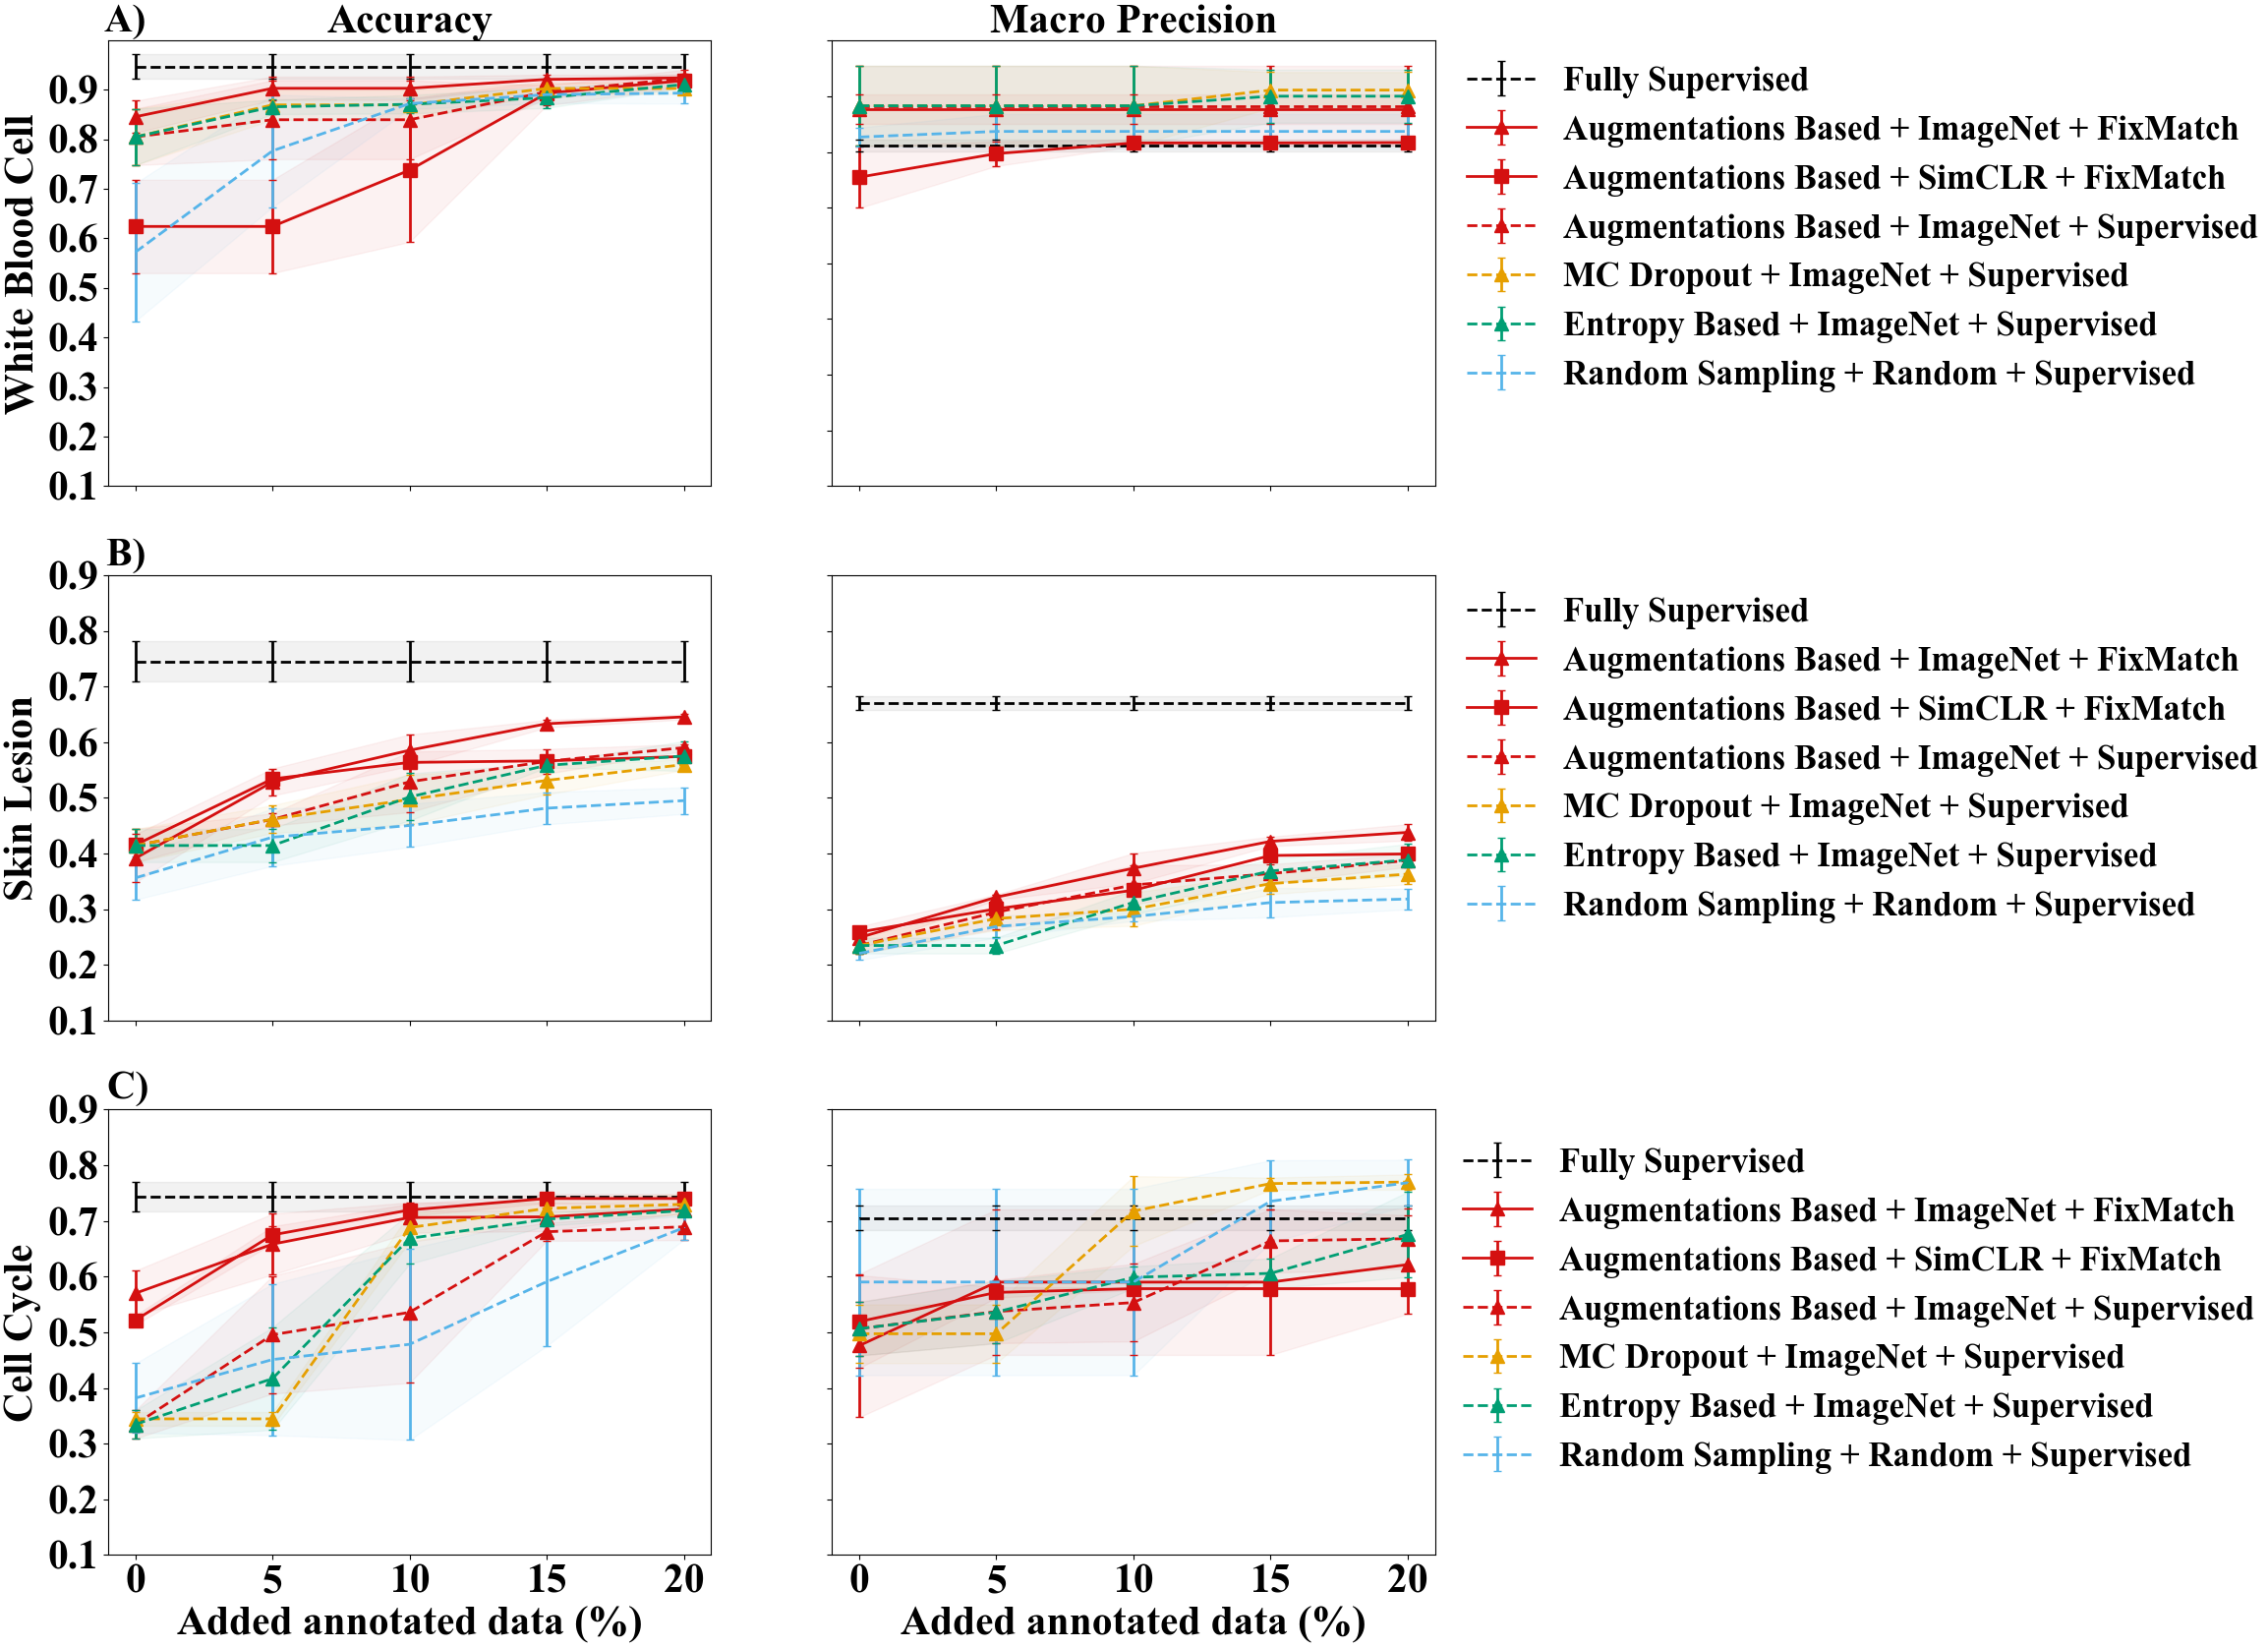
\includegraphics[width=\textwidth]{figures/fig_3_acc_precision.png}
\caption{The combination of augmentation-based sampling, SimCLR or ImageNet pre-training and semi-supervised training with FixMatch is the optimal strategy on all three biomedical datasets. Mean $\pm$ standard deviation of the macro recall are shown after 4-fold cross-validation. (A) On the white blood cell dataset the optimal strategy with ImageNet initialization outperformed all other baseline methods for each active learning iteration by at least 3\%. With only 20\% of added annotated data, this combination performs almost as good as a fully supervised trained model. (B) On the skin lesion dataset the optimal strategies with ImageNet and SimCLR pre-training outperformed all other methods. During the initial step (no added data) and 5\% added data (first iteration), both optimal strategies were at least 4\% better than all baseline methods. (C) On the cell cycle dataset the optimal strategies with ImageNet and SimCLR pre-training were ~14\% better than all baseline methods with no added data. Nonetheless, the optimal strategy with ImageNet pre-training did not improve as rapidly as the optimal strategy with SimCLR pre-training. The optimal strategy with SimCLR pre-training was ~3\% better than all baseline methods and only 6\% worse than the fully supervised trained model, however using only 20\% of annotated data.}
\label{fig:all_acc_precision}
\end{figure}

\begin{figure}[htbp]
\centering
\captionsetup{format=plain}
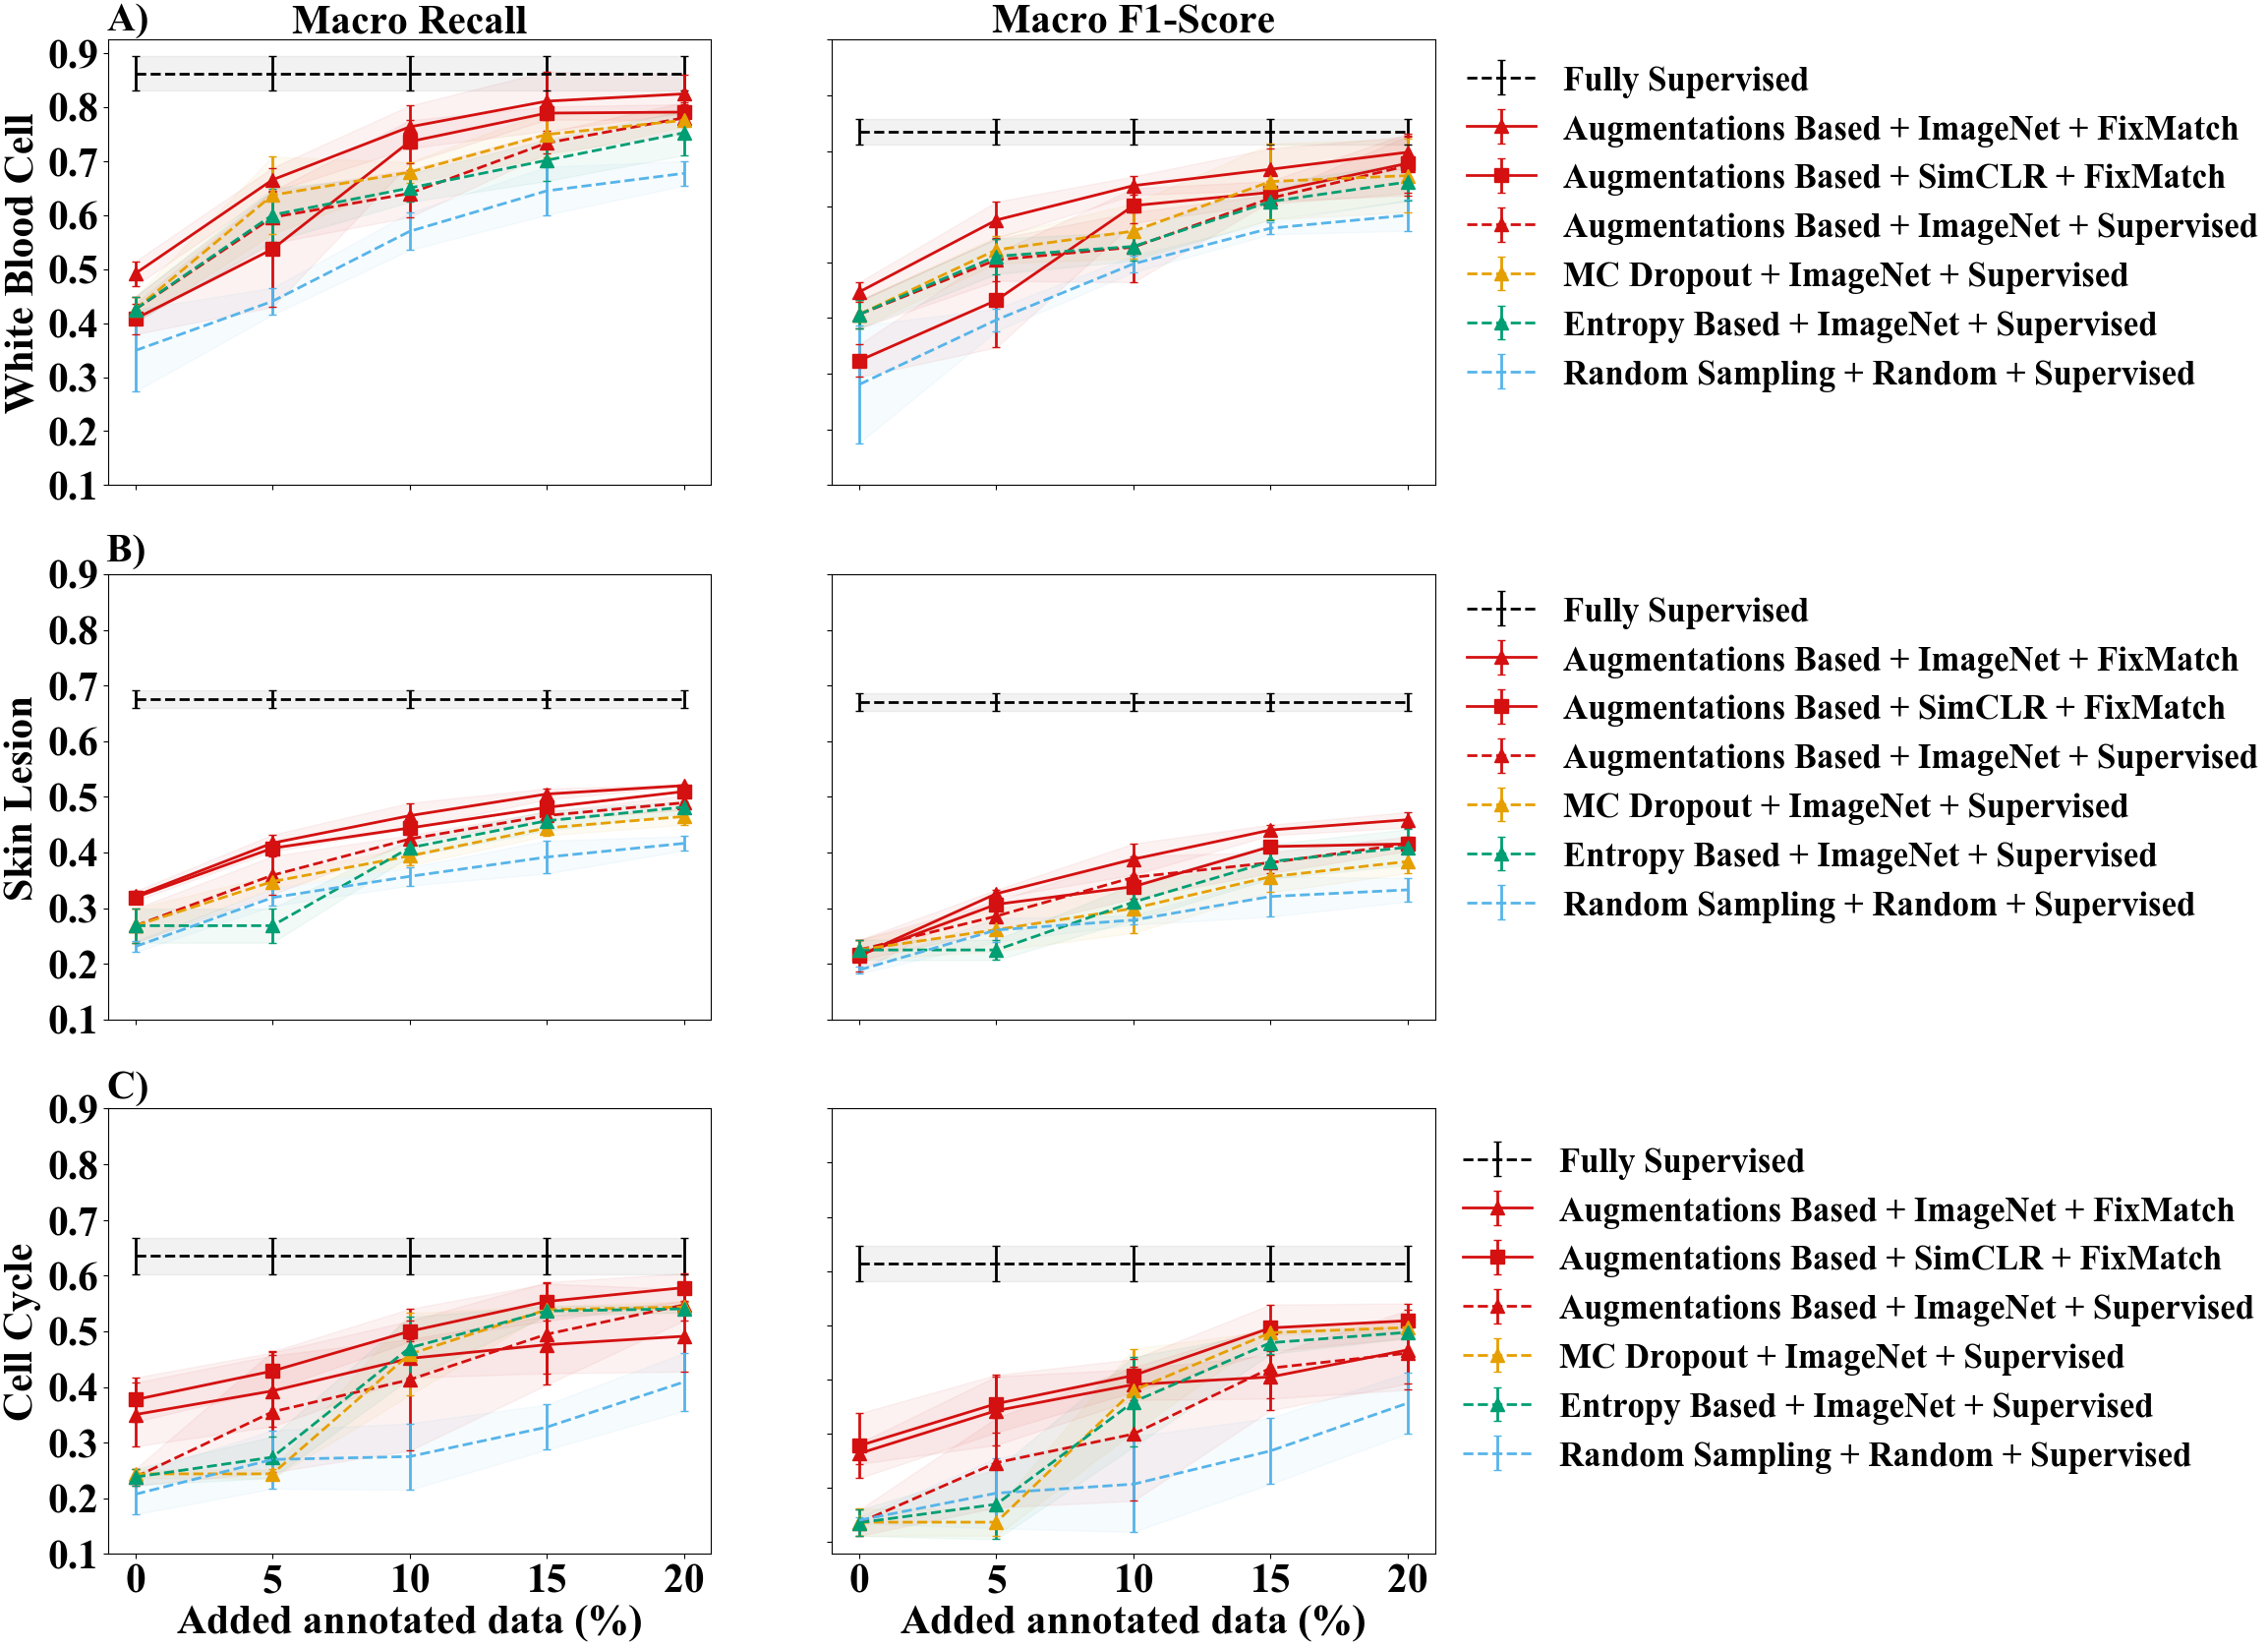
\includegraphics[width=\textwidth]{figures/fig_3_recall_f1.png}
\caption{The combination of augmentation-based sampling, SimCLR or ImageNet pre-training and semi-supervised training with FixMatch is the optimal strategy on all three biomedical datasets. Mean $\pm$ standard deviation of the macro recall are shown after 4-fold cross-validation. (A) On the white blood cell dataset the optimal strategy with ImageNet initialization outperformed all other baseline methods for each active learning iteration by at least 3\%. With only 20\% of added annotated data, this combination performs almost as good as a fully supervised trained model. (B) On the skin lesion dataset the optimal strategies with ImageNet and SimCLR pre-training outperformed all other methods. During the initial step (no added data) and 5\% added data (first iteration), both optimal strategies were at least 4\% better than all baseline methods. (C) On the cell cycle dataset the optimal strategies with ImageNet and SimCLR pre-training were ~14\% better than all baseline methods with no added data. Nonetheless, the optimal strategy with ImageNet pre-training did not improve as rapidly as the optimal strategy with SimCLR pre-training. The optimal strategy with SimCLR pre-training was ~3\% better than all baseline methods and only 6\% worse than the fully supervised trained model, however using only 20\% of annotated data.}
\label{fig:all_recall_f1}
\end{figure}

\newpage

\section{Recommended strategy}
As a result of the previous sections, the optimal strategy is identified as the combination of augmentation-based sampling, ImageNet/SimCLR pre-training and FixMatch to show the best results on 3 biomedical datasets. As illustrated in Figure 3, the ImageNet pre-training works better for white blood cells and the skin lesions from the initial step. SimCLR pre-training seems to work best on the cell cycle data. Therefore, the recommended strategy is to find the best pre-training method on the initial step and combine it with augmentation-based sampling and FixMatch during training. The results of the recommended strategy improves macro recall by 4\% for white blood cells data, 3\% on skin lesions data and 3\% for cell cycle data on the last iteration, with respect to the best conventional active learning method for each dataset.

\begin{figure}[htbp]
\centering
\captionsetup{format=plain}
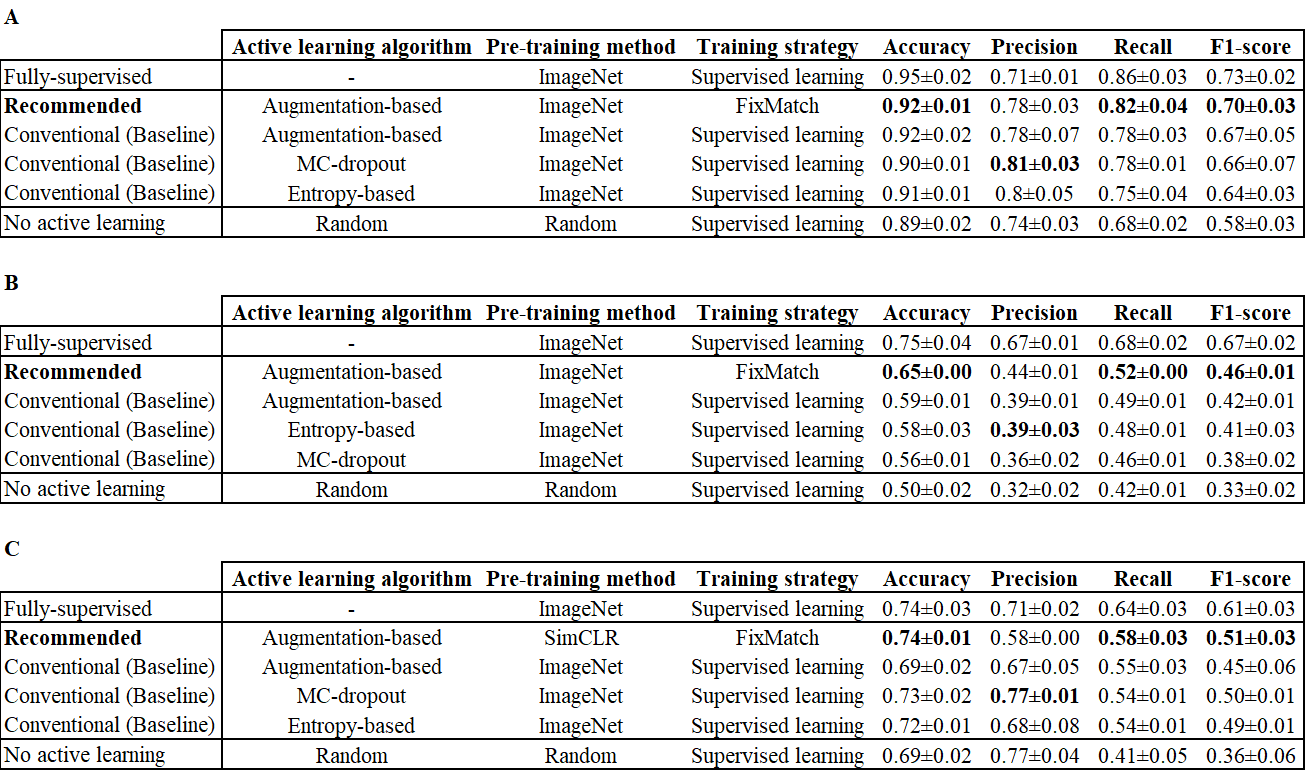
\includegraphics[width=\textwidth]{figures/fig_results_3.png}
\caption{Comparing the results of the last iteration, the recommended strategies outperform conventional annotation-efficient learning. (A) On the white blood cell dataset, the combination of augmentation-based sampling, ImageNet pretraining and FixMatch training brings an improvement of 4\% on macro recall and 3\% on F1-score over the highest baseline. With using only 20\% of added labeled data, this strategy is only 4\% lower in recall and 3\% lower with respect to the F1-score as compared to fully-supervised training. (B) On the skin lesions dataset, the recommended strategy brings an improvement of 3\% on macro recall, 5\% improvement on precision and 6\% on F1-score. The high recall difference to the fully-supervised results shows that the amount of labeled data was not enough and more iterations were needed. (C) On the cell cycle dataset, the recommended strategy brings an improvement of 3\% on recall and 6\% on F1-score.
}
\label{fig:results_3}
\end{figure}